\documentclass{article}

\usepackage{iclr2025_conference,times}
%%%%% NEW MATH DEFINITIONS %%%%%

\usepackage{amsmath,amsfonts,bm}

% Mark sections of captions for referring to divisions of figures
\newcommand{\figleft}{{\em (Left)}}
\newcommand{\figcenter}{{\em (Center)}}
\newcommand{\figright}{{\em (Right)}}
\newcommand{\figtop}{{\em (Top)}}
\newcommand{\figbottom}{{\em (Bottom)}}
\newcommand{\captiona}{{\em (a)}}
\newcommand{\captionb}{{\em (b)}}
\newcommand{\captionc}{{\em (c)}}
\newcommand{\captiond}{{\em (d)}}

% Highlight a newly defined term
\newcommand{\newterm}[1]{{\bf #1}}


% Figure reference, lower-case.
\def\figref#1{figure~\ref{#1}}
% Figure reference, capital. For start of sentence
\def\Figref#1{Figure~\ref{#1}}
\def\twofigref#1#2{figures \ref{#1} and \ref{#2}}
\def\quadfigref#1#2#3#4{figures \ref{#1}, \ref{#2}, \ref{#3} and \ref{#4}}
% Section reference, lower-case.
\def\secref#1{section~\ref{#1}}
% Section reference, capital.
\def\Secref#1{Section~\ref{#1}}
% Reference to two sections.
\def\twosecrefs#1#2{sections \ref{#1} and \ref{#2}}
% Reference to three sections.
\def\secrefs#1#2#3{sections \ref{#1}, \ref{#2} and \ref{#3}}
% Reference to an equation, lower-case.
\def\eqref#1{equation~\ref{#1}}
% Reference to an equation, upper case
\def\Eqref#1{Equation~\ref{#1}}
% A raw reference to an equation---avoid using if possible
\def\plaineqref#1{\ref{#1}}
% Reference to a chapter, lower-case.
\def\chapref#1{chapter~\ref{#1}}
% Reference to an equation, upper case.
\def\Chapref#1{Chapter~\ref{#1}}
% Reference to a range of chapters
\def\rangechapref#1#2{chapters\ref{#1}--\ref{#2}}
% Reference to an algorithm, lower-case.
\def\algref#1{algorithm~\ref{#1}}
% Reference to an algorithm, upper case.
\def\Algref#1{Algorithm~\ref{#1}}
\def\twoalgref#1#2{algorithms \ref{#1} and \ref{#2}}
\def\Twoalgref#1#2{Algorithms \ref{#1} and \ref{#2}}
% Reference to a part, lower case
\def\partref#1{part~\ref{#1}}
% Reference to a part, upper case
\def\Partref#1{Part~\ref{#1}}
\def\twopartref#1#2{parts \ref{#1} and \ref{#2}}

\def\ceil#1{\lceil #1 \rceil}
\def\floor#1{\lfloor #1 \rfloor}
\def\1{\bm{1}}
\newcommand{\train}{\mathcal{D}}
\newcommand{\valid}{\mathcal{D_{\mathrm{valid}}}}
\newcommand{\test}{\mathcal{D_{\mathrm{test}}}}

\def\eps{{\epsilon}}


% Random variables
\def\reta{{\textnormal{$\eta$}}}
\def\ra{{\textnormal{a}}}
\def\rb{{\textnormal{b}}}
\def\rc{{\textnormal{c}}}
\def\rd{{\textnormal{d}}}
\def\re{{\textnormal{e}}}
\def\rf{{\textnormal{f}}}
\def\rg{{\textnormal{g}}}
\def\rh{{\textnormal{h}}}
\def\ri{{\textnormal{i}}}
\def\rj{{\textnormal{j}}}
\def\rk{{\textnormal{k}}}
\def\rl{{\textnormal{l}}}
% rm is already a command, just don't name any random variables m
\def\rn{{\textnormal{n}}}
\def\ro{{\textnormal{o}}}
\def\rp{{\textnormal{p}}}
\def\rq{{\textnormal{q}}}
\def\rr{{\textnormal{r}}}
\def\rs{{\textnormal{s}}}
\def\rt{{\textnormal{t}}}
\def\ru{{\textnormal{u}}}
\def\rv{{\textnormal{v}}}
\def\rw{{\textnormal{w}}}
\def\rx{{\textnormal{x}}}
\def\ry{{\textnormal{y}}}
\def\rz{{\textnormal{z}}}

% Random vectors
\def\rvepsilon{{\mathbf{\epsilon}}}
\def\rvtheta{{\mathbf{\theta}}}
\def\rva{{\mathbf{a}}}
\def\rvb{{\mathbf{b}}}
\def\rvc{{\mathbf{c}}}
\def\rvd{{\mathbf{d}}}
\def\rve{{\mathbf{e}}}
\def\rvf{{\mathbf{f}}}
\def\rvg{{\mathbf{g}}}
\def\rvh{{\mathbf{h}}}
\def\rvu{{\mathbf{i}}}
\def\rvj{{\mathbf{j}}}
\def\rvk{{\mathbf{k}}}
\def\rvl{{\mathbf{l}}}
\def\rvm{{\mathbf{m}}}
\def\rvn{{\mathbf{n}}}
\def\rvo{{\mathbf{o}}}
\def\rvp{{\mathbf{p}}}
\def\rvq{{\mathbf{q}}}
\def\rvr{{\mathbf{r}}}
\def\rvs{{\mathbf{s}}}
\def\rvt{{\mathbf{t}}}
\def\rvu{{\mathbf{u}}}
\def\rvv{{\mathbf{v}}}
\def\rvw{{\mathbf{w}}}
\def\rvx{{\mathbf{x}}}
\def\rvy{{\mathbf{y}}}
\def\rvz{{\mathbf{z}}}

% Elements of random vectors
\def\erva{{\textnormal{a}}}
\def\ervb{{\textnormal{b}}}
\def\ervc{{\textnormal{c}}}
\def\ervd{{\textnormal{d}}}
\def\erve{{\textnormal{e}}}
\def\ervf{{\textnormal{f}}}
\def\ervg{{\textnormal{g}}}
\def\ervh{{\textnormal{h}}}
\def\ervi{{\textnormal{i}}}
\def\ervj{{\textnormal{j}}}
\def\ervk{{\textnormal{k}}}
\def\ervl{{\textnormal{l}}}
\def\ervm{{\textnormal{m}}}
\def\ervn{{\textnormal{n}}}
\def\ervo{{\textnormal{o}}}
\def\ervp{{\textnormal{p}}}
\def\ervq{{\textnormal{q}}}
\def\ervr{{\textnormal{r}}}
\def\ervs{{\textnormal{s}}}
\def\ervt{{\textnormal{t}}}
\def\ervu{{\textnormal{u}}}
\def\ervv{{\textnormal{v}}}
\def\ervw{{\textnormal{w}}}
\def\ervx{{\textnormal{x}}}
\def\ervy{{\textnormal{y}}}
\def\ervz{{\textnormal{z}}}

% Random matrices
\def\rmA{{\mathbf{A}}}
\def\rmB{{\mathbf{B}}}
\def\rmC{{\mathbf{C}}}
\def\rmD{{\mathbf{D}}}
\def\rmE{{\mathbf{E}}}
\def\rmF{{\mathbf{F}}}
\def\rmG{{\mathbf{G}}}
\def\rmH{{\mathbf{H}}}
\def\rmI{{\mathbf{I}}}
\def\rmJ{{\mathbf{J}}}
\def\rmK{{\mathbf{K}}}
\def\rmL{{\mathbf{L}}}
\def\rmM{{\mathbf{M}}}
\def\rmN{{\mathbf{N}}}
\def\rmO{{\mathbf{O}}}
\def\rmP{{\mathbf{P}}}
\def\rmQ{{\mathbf{Q}}}
\def\rmR{{\mathbf{R}}}
\def\rmS{{\mathbf{S}}}
\def\rmT{{\mathbf{T}}}
\def\rmU{{\mathbf{U}}}
\def\rmV{{\mathbf{V}}}
\def\rmW{{\mathbf{W}}}
\def\rmX{{\mathbf{X}}}
\def\rmY{{\mathbf{Y}}}
\def\rmZ{{\mathbf{Z}}}

% Elements of random matrices
\def\ermA{{\textnormal{A}}}
\def\ermB{{\textnormal{B}}}
\def\ermC{{\textnormal{C}}}
\def\ermD{{\textnormal{D}}}
\def\ermE{{\textnormal{E}}}
\def\ermF{{\textnormal{F}}}
\def\ermG{{\textnormal{G}}}
\def\ermH{{\textnormal{H}}}
\def\ermI{{\textnormal{I}}}
\def\ermJ{{\textnormal{J}}}
\def\ermK{{\textnormal{K}}}
\def\ermL{{\textnormal{L}}}
\def\ermM{{\textnormal{M}}}
\def\ermN{{\textnormal{N}}}
\def\ermO{{\textnormal{O}}}
\def\ermP{{\textnormal{P}}}
\def\ermQ{{\textnormal{Q}}}
\def\ermR{{\textnormal{R}}}
\def\ermS{{\textnormal{S}}}
\def\ermT{{\textnormal{T}}}
\def\ermU{{\textnormal{U}}}
\def\ermV{{\textnormal{V}}}
\def\ermW{{\textnormal{W}}}
\def\ermX{{\textnormal{X}}}
\def\ermY{{\textnormal{Y}}}
\def\ermZ{{\textnormal{Z}}}

% Vectors
\def\vzero{{\bm{0}}}
\def\vone{{\bm{1}}}
\def\vmu{{\bm{\mu}}}
\def\vtheta{{\bm{\theta}}}
\def\va{{\bm{a}}}
\def\vb{{\bm{b}}}
\def\vc{{\bm{c}}}
\def\vd{{\bm{d}}}
\def\ve{{\bm{e}}}
\def\vf{{\bm{f}}}
\def\vg{{\bm{g}}}
\def\vh{{\bm{h}}}
\def\vi{{\bm{i}}}
\def\vj{{\bm{j}}}
\def\vk{{\bm{k}}}
\def\vl{{\bm{l}}}
\def\vm{{\bm{m}}}
\def\vn{{\bm{n}}}
\def\vo{{\bm{o}}}
\def\vp{{\bm{p}}}
\def\vq{{\bm{q}}}
\def\vr{{\bm{r}}}
\def\vs{{\bm{s}}}
\def\vt{{\bm{t}}}
\def\vu{{\bm{u}}}
\def\vv{{\bm{v}}}
\def\vw{{\bm{w}}}
\def\vx{{\bm{x}}}
\def\vy{{\bm{y}}}
\def\vz{{\bm{z}}}

% Elements of vectors
\def\evalpha{{\alpha}}
\def\evbeta{{\beta}}
\def\evepsilon{{\epsilon}}
\def\evlambda{{\lambda}}
\def\evomega{{\omega}}
\def\evmu{{\mu}}
\def\evpsi{{\psi}}
\def\evsigma{{\sigma}}
\def\evtheta{{\theta}}
\def\eva{{a}}
\def\evb{{b}}
\def\evc{{c}}
\def\evd{{d}}
\def\eve{{e}}
\def\evf{{f}}
\def\evg{{g}}
\def\evh{{h}}
\def\evi{{i}}
\def\evj{{j}}
\def\evk{{k}}
\def\evl{{l}}
\def\evm{{m}}
\def\evn{{n}}
\def\evo{{o}}
\def\evp{{p}}
\def\evq{{q}}
\def\evr{{r}}
\def\evs{{s}}
\def\evt{{t}}
\def\evu{{u}}
\def\evv{{v}}
\def\evw{{w}}
\def\evx{{x}}
\def\evy{{y}}
\def\evz{{z}}

% Matrix
\def\mA{{\bm{A}}}
\def\mB{{\bm{B}}}
\def\mC{{\bm{C}}}
\def\mD{{\bm{D}}}
\def\mE{{\bm{E}}}
\def\mF{{\bm{F}}}
\def\mG{{\bm{G}}}
\def\mH{{\bm{H}}}
\def\mI{{\bm{I}}}
\def\mJ{{\bm{J}}}
\def\mK{{\bm{K}}}
\def\mL{{\bm{L}}}
\def\mM{{\bm{M}}}
\def\mN{{\bm{N}}}
\def\mO{{\bm{O}}}
\def\mP{{\bm{P}}}
\def\mQ{{\bm{Q}}}
\def\mR{{\bm{R}}}
\def\mS{{\bm{S}}}
\def\mT{{\bm{T}}}
\def\mU{{\bm{U}}}
\def\mV{{\bm{V}}}
\def\mW{{\bm{W}}}
\def\mX{{\bm{X}}}
\def\mY{{\bm{Y}}}
\def\mZ{{\bm{Z}}}
\def\mBeta{{\bm{\beta}}}
\def\mPhi{{\bm{\Phi}}}
\def\mLambda{{\bm{\Lambda}}}
\def\mSigma{{\bm{\Sigma}}}

% Tensor
\DeclareMathAlphabet{\mathsfit}{\encodingdefault}{\sfdefault}{m}{sl}
\SetMathAlphabet{\mathsfit}{bold}{\encodingdefault}{\sfdefault}{bx}{n}
\newcommand{\tens}[1]{\bm{\mathsfit{#1}}}
\def\tA{{\tens{A}}}
\def\tB{{\tens{B}}}
\def\tC{{\tens{C}}}
\def\tD{{\tens{D}}}
\def\tE{{\tens{E}}}
\def\tF{{\tens{F}}}
\def\tG{{\tens{G}}}
\def\tH{{\tens{H}}}
\def\tI{{\tens{I}}}
\def\tJ{{\tens{J}}}
\def\tK{{\tens{K}}}
\def\tL{{\tens{L}}}
\def\tM{{\tens{M}}}
\def\tN{{\tens{N}}}
\def\tO{{\tens{O}}}
\def\tP{{\tens{P}}}
\def\tQ{{\tens{Q}}}
\def\tR{{\tens{R}}}
\def\tS{{\tens{S}}}
\def\tT{{\tens{T}}}
\def\tU{{\tens{U}}}
\def\tV{{\tens{V}}}
\def\tW{{\tens{W}}}
\def\tX{{\tens{X}}}
\def\tY{{\tens{Y}}}
\def\tZ{{\tens{Z}}}


% Graph
\def\gA{{\mathcal{A}}}
\def\gB{{\mathcal{B}}}
\def\gC{{\mathcal{C}}}
\def\gD{{\mathcal{D}}}
\def\gE{{\mathcal{E}}}
\def\gF{{\mathcal{F}}}
\def\gG{{\mathcal{G}}}
\def\gH{{\mathcal{H}}}
\def\gI{{\mathcal{I}}}
\def\gJ{{\mathcal{J}}}
\def\gK{{\mathcal{K}}}
\def\gL{{\mathcal{L}}}
\def\gM{{\mathcal{M}}}
\def\gN{{\mathcal{N}}}
\def\gO{{\mathcal{O}}}
\def\gP{{\mathcal{P}}}
\def\gQ{{\mathcal{Q}}}
\def\gR{{\mathcal{R}}}
\def\gS{{\mathcal{S}}}
\def\gT{{\mathcal{T}}}
\def\gU{{\mathcal{U}}}
\def\gV{{\mathcal{V}}}
\def\gW{{\mathcal{W}}}
\def\gX{{\mathcal{X}}}
\def\gY{{\mathcal{Y}}}
\def\gZ{{\mathcal{Z}}}

% Sets
\def\sA{{\mathbb{A}}}
\def\sB{{\mathbb{B}}}
\def\sC{{\mathbb{C}}}
\def\sD{{\mathbb{D}}}
% Don't use a set called E, because this would be the same as our symbol
% for expectation.
\def\sF{{\mathbb{F}}}
\def\sG{{\mathbb{G}}}
\def\sH{{\mathbb{H}}}
\def\sI{{\mathbb{I}}}
\def\sJ{{\mathbb{J}}}
\def\sK{{\mathbb{K}}}
\def\sL{{\mathbb{L}}}
\def\sM{{\mathbb{M}}}
\def\sN{{\mathbb{N}}}
\def\sO{{\mathbb{O}}}
\def\sP{{\mathbb{P}}}
\def\sQ{{\mathbb{Q}}}
\def\sR{{\mathbb{R}}}
\def\sS{{\mathbb{S}}}
\def\sT{{\mathbb{T}}}
\def\sU{{\mathbb{U}}}
\def\sV{{\mathbb{V}}}
\def\sW{{\mathbb{W}}}
\def\sX{{\mathbb{X}}}
\def\sY{{\mathbb{Y}}}
\def\sZ{{\mathbb{Z}}}

% Entries of a matrix
\def\emLambda{{\Lambda}}
\def\emA{{A}}
\def\emB{{B}}
\def\emC{{C}}
\def\emD{{D}}
\def\emE{{E}}
\def\emF{{F}}
\def\emG{{G}}
\def\emH{{H}}
\def\emI{{I}}
\def\emJ{{J}}
\def\emK{{K}}
\def\emL{{L}}
\def\emM{{M}}
\def\emN{{N}}
\def\emO{{O}}
\def\emP{{P}}
\def\emQ{{Q}}
\def\emR{{R}}
\def\emS{{S}}
\def\emT{{T}}
\def\emU{{U}}
\def\emV{{V}}
\def\emW{{W}}
\def\emX{{X}}
\def\emY{{Y}}
\def\emZ{{Z}}
\def\emSigma{{\Sigma}}

% entries of a tensor
% Same font as tensor, without \bm wrapper
\newcommand{\etens}[1]{\mathsfit{#1}}
\def\etLambda{{\etens{\Lambda}}}
\def\etA{{\etens{A}}}
\def\etB{{\etens{B}}}
\def\etC{{\etens{C}}}
\def\etD{{\etens{D}}}
\def\etE{{\etens{E}}}
\def\etF{{\etens{F}}}
\def\etG{{\etens{G}}}
\def\etH{{\etens{H}}}
\def\etI{{\etens{I}}}
\def\etJ{{\etens{J}}}
\def\etK{{\etens{K}}}
\def\etL{{\etens{L}}}
\def\etM{{\etens{M}}}
\def\etN{{\etens{N}}}
\def\etO{{\etens{O}}}
\def\etP{{\etens{P}}}
\def\etQ{{\etens{Q}}}
\def\etR{{\etens{R}}}
\def\etS{{\etens{S}}}
\def\etT{{\etens{T}}}
\def\etU{{\etens{U}}}
\def\etV{{\etens{V}}}
\def\etW{{\etens{W}}}
\def\etX{{\etens{X}}}
\def\etY{{\etens{Y}}}
\def\etZ{{\etens{Z}}}

% The true underlying data generating distribution
\newcommand{\pdata}{p_{\rm{data}}}
% The empirical distribution defined by the training set
\newcommand{\ptrain}{\hat{p}_{\rm{data}}}
\newcommand{\Ptrain}{\hat{P}_{\rm{data}}}
% The model distribution
\newcommand{\pmodel}{p_{\rm{model}}}
\newcommand{\Pmodel}{P_{\rm{model}}}
\newcommand{\ptildemodel}{\tilde{p}_{\rm{model}}}
% Stochastic autoencoder distributions
\newcommand{\pencode}{p_{\rm{encoder}}}
\newcommand{\pdecode}{p_{\rm{decoder}}}
\newcommand{\precons}{p_{\rm{reconstruct}}}

\newcommand{\laplace}{\mathrm{Laplace}} % Laplace distribution

\newcommand{\E}{\mathbb{E}}
\newcommand{\Ls}{\mathcal{L}}
\newcommand{\R}{\mathbb{R}}
\newcommand{\emp}{\tilde{p}}
\newcommand{\lr}{\alpha}
\newcommand{\reg}{\lambda}
\newcommand{\rect}{\mathrm{rectifier}}
\newcommand{\softmax}{\mathrm{softmax}}
\newcommand{\sigmoid}{\sigma}
\newcommand{\softplus}{\zeta}
\newcommand{\KL}{D_{\mathrm{KL}}}
\newcommand{\Var}{\mathrm{Var}}
\newcommand{\standarderror}{\mathrm{SE}}
\newcommand{\Cov}{\mathrm{Cov}}
% Wolfram Mathworld says $L^2$ is for function spaces and $\ell^2$ is for vectors
% But then they seem to use $L^2$ for vectors throughout the site, and so does
% wikipedia.
\newcommand{\normlzero}{L^0}
\newcommand{\normlone}{L^1}
\newcommand{\normltwo}{L^2}
\newcommand{\normlp}{L^p}
\newcommand{\normmax}{L^\infty}

\newcommand{\parents}{Pa} % See usage in notation.tex. Chosen to match Daphne's book.

\DeclareMathOperator*{\argmax}{arg\,max}
\DeclareMathOperator*{\argmin}{arg\,min}

\DeclareMathOperator{\sign}{sign}
\DeclareMathOperator{\Tr}{Tr}
\let\ab\allowbreak


\usepackage{hyperref}
\usepackage{url}
\usepackage{graphicx}
\usepackage{booktabs}
\usepackage{multirow}
\usepackage{microtype}
\usepackage{enumitem}
\usepackage{xcolor}
\usepackage{amsmath}
\usepackage{amssymb}
\usepackage{placeins}
\usepackage{longtable}
\hypersetup{hidelinks}

\definecolor{supported}{RGB}{46,108,74}
\definecolor{warning}{RGB}{166,92,31}
\definecolor{rejected}{RGB}{145,47,47}

\newcommand{\system}{\textsc{RunForest}}
\newcommand{\ours}{Decision Admissibility}
\newcommand{\clean}{\textsc{Clean}}
\newcommand{\blocked}{\textsc{Blocked}}
\newcommand{\protocolbiased}{\textsc{Protocol-Biased}}
\newcommand{\rankeligible}{\textsc{Rank-Eligible}}
\newcommand{\todoresult}[1]{\textcolor{warning}{[#1]}}

\title{Relevance Is Not Authority:\\
Decision Admissibility for Recursive Machine Learning Agents}

\author{Anonymous authors\\
Paper under double-blind review}

% Uncomment only for the camera-ready version.
% \iclrfinalcopy

\begin{document}

\maketitle

\begin{abstract}
Recursive machine-learning engineering (MLE) agents reuse code, scores,
failures, and distilled procedures, yet relevance is not authority.  A single
experience may contain a useful repair, a genuinely executed program, and a
statistically invalid score; an item-level valid bit must either expose the
invalid claim or discard the useful one.  We present \ours{}, which governs the
atomic unit $(\text{claim},\text{operation},\text{generation stage},
\text{governance stage},\text{protocol},\text{task})$.  A stage/granularity gate
first proposes RunForest or SOP-clause evidence.  A protocol-compiled authority
gate then removes unauthorized clauses before ranking, token competition, and
prompt construction.  Host-owned execution receipts first authorize the
current node's independent Result Fact.  Separate static/runtime and
counterfactual receipts then authorize Adoption and Causal Edges from a
historical experience to that node; absence of such an edge does not erase a
protocol-legal result.  Immutable Base-Bundle and append-only Overlay
publication prevent descendant authority from expanding through summaries or
writeback.  A method-preserving Clean
Replay creates a new support path rather than rewriting polluted history.
The implemented deterministic suite retains both legal Debug clauses in a
mixed-value example while producing zero unauthorized prompt exposure and
suppressing its contaminated score from Rank.  A separately built non-Spooky
corpus contains 79 complete runs across 16 tasks, 1,577 audited code nodes, and
1,545 bound clauses; raw-audited bundles intentionally contain zero certified
adoption edges.  In a prospective audit of 12 verified natural run packets,
the gate automatically suppresses 783 of 4,106 raw candidates (19.07\%) before
prompt construction; a separately reported known-invalid control is proposed
once and exposed zero times.  This is an automatic suppression rate, not an
independently adjudicated invalid-memory prevalence.  Existing retrospective
routing diagnostics remain positive:
the dynamic Debug route reaches 0.800 route accuracy and 0.760 selective
decision accuracy on a fixed 25-episode test partition.  The corrected shadow/canary, controlled $2\times2$, multi-generation,
and formal same-domain task-heldout evaluations are complete and hash-bound.
Across nine task--seed blocks, all 45 online assignments were retained: Full
Decision Admissibility completed 4/9 versus 6/9 for No Memory.  The four
score-estimable pairs all favored Full, but the exact one-sided sign-flip
$p=0.0625$, Holm-adjusted $p=0.25$, zero estimable Taxi pairs, and poorer
completion reject the frozen superiority claim.  We therefore claim engineering
and admissibility invariants, not improved final MLE performance or
experience-level causality.
\end{abstract}

\section{Introduction}

MLE agents must choose data protocols, model families, optimization settings,
and debugging actions while repeatedly generating and executing code.  Systems
such as AIDE organize this process as search over programs
\citep{jiang2025aide}, and MLE-Bench provides a standardized collection of
Kaggle-style tasks for evaluation \citep{chan2024mlebench}.  Recent work shows
that rich execution feedback and persistent experience can direct later
updates \citep{zhang2026gome}, while procedural-memory systems distill and
retrieve reusable skills \citep{xia2026skillrl,li2026skillgraph}.

The central difficulty in executable MLE is not only whether memory is
relevant.  It is whether a particular claim inside an experience is
\emph{admissible} for the current operation and protocol, and whether it
actually changes the resulting program.  Consider a
program that combines a Transformer, TF--IDF models, and learned ensemble
weights.  Its architecture may be valuable while its reported score is invalid
because a vectorizer saw the report set or because weights were selected and
reported on the same labels.  Blindly replaying the program promotes invalid
evidence.  Dropping it discards potentially useful method structure.  Asking a
general debugging agent to repair it may silently replace the model, shrink the
training budget, or introduce a second protocol error.

We study this failure as an influence-governance problem in recursive
improvement:

\begin{quote}
Which atomic claims may influence a particular learning operation under the
active protocol, how can that influence be verified, and what may propagate to
future descendants?
\end{quote}

Our answer is \ours{}, implemented in \system{}.  Figure~\ref{fig:architecture}
summarizes one experience-influence transaction: propose a stage-compatible
representation, admit legal claim--use pairs before they can affect ranking or
the prompt, execute the current artifact and publish its own legal Result Fact,
then optionally certify historical Adoption or Causal influence with
contract-bound host receipts.  Each object is committed separately and cannot
expand its supported scope.
RunForest is the immutable evidence view; SOP clauses are the actionable view;
Dynamic Hybrid is a proposal policy rather than the authority mechanism.

\begin{figure*}[t]
  \centering
  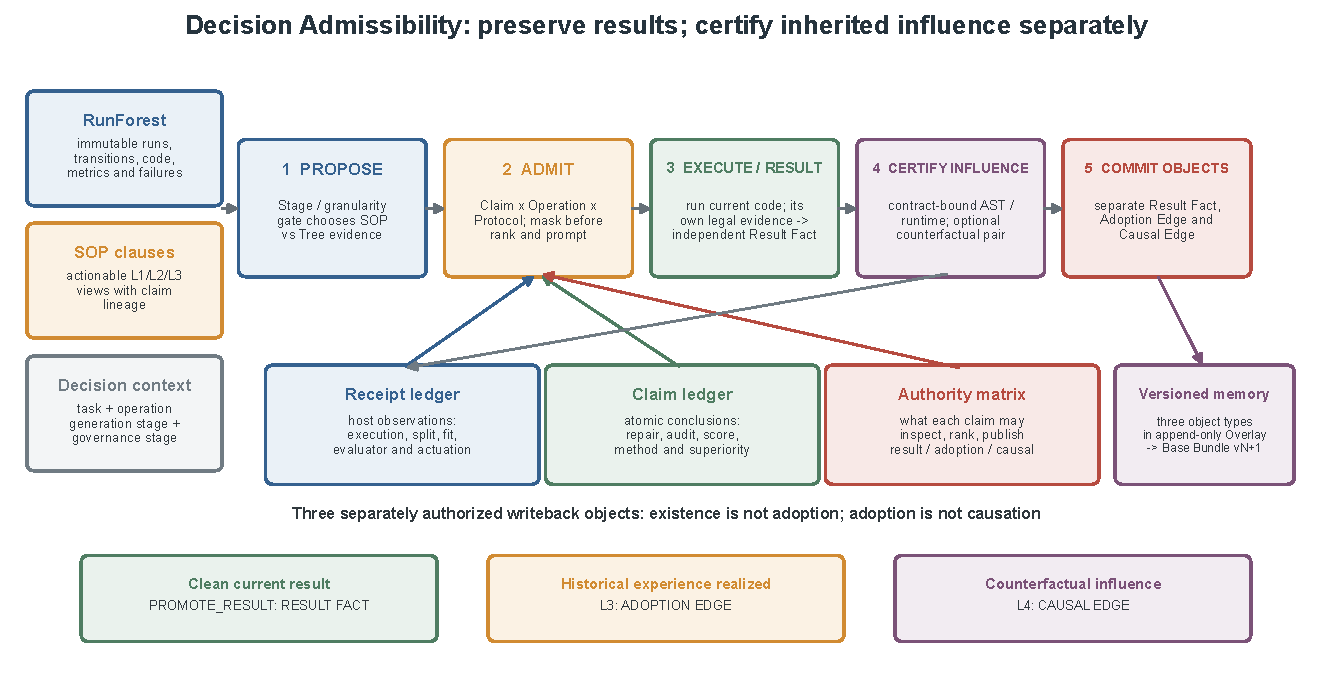
\includegraphics[width=\textwidth]{figures/architecture.pdf}
  \caption{\textbf{Decision Admissibility as one influence transaction.}
  RunForest and SOP clauses provide evidence and actionable views.  The system
  proposes stage-compatible claims and authorizes each Claim--Operation pair
  before ranking and prompting.  A legal current execution may publish a Result
  Fact independently; contract-bound static/runtime evidence publishes an
  Adoption Edge, and counterfactual evidence publishes a Causal Edge.  The three
  append-only objects have separate permissions.}
  \label{fig:architecture}
\end{figure*}

This draft makes three deliberately scoped contributions:

\begin{enumerate}[leftmargin=*,itemsep=2pt]
  \item \textbf{Claim-use formulation.}  We separate retrieval relevance, use
  authority, and realized actuation, and make the governed object an atomic
  Claim--Operation pair under two stage axes and an active ProtocolSpec.
  \item \textbf{Pre-use/post-use transaction.}  We combine stage-aware
  proposal, clause-level pre-prompt authority, host-owned receipts, and
  method-preserving Clean Replay with three non-conflated writeback objects:
  independently supported Result Facts, realized Adoption Edges, and
  counterfactually supported Causal Edges.
  \item \textbf{Executable evidence boundary.}  We provide deterministic
  mixed-value, bypass, replay-identity, immutable-publication, and rollback
  tests, split-isolated real-corpus bundles, controlled IIR--VKR and
  multi-generation evaluations, a prospective dual-observer audit, and a
  preregistered same-domain online study.  The prospective audit measures
  pre-prompt gate activity without equating automatic suppression with Oracle
  invalidity; the formal study preserves all failures and rejects, rather than
  launders, the Full-over-No-Memory superiority claim.
\end{enumerate}

We deliberately do \emph{not} claim that the current system improves downstream
MLE scores, that a RunForest edge is itself causal, or that hyperbolic geometry
is superior.  The evidence now establishes implementation invariants,
split-isolated bundle construction, controlled safety--utility mechanisms, and
formal execution integrity.  The preregistered online comparison rejects Full
superiority; conditional positive deltas remain diagnostic, and experience
causality remains pending without L4 counterfactual receipts for the formal
gains.

\section{Related Work}

\paragraph{MLE agents and execution-guided search.}
AIDE searches a tree of executable code variants \citep{jiang2025aide};
MLE-Bench evaluates agents on realistic competition tasks
\citep{chan2024mlebench}.  GOME uses structured diagnostics as a gradient and
success memory as momentum \citep{zhang2026gome}.  Our focus is orthogonal to
the update operator: before an experience can guide an update, we ask whether
its abstraction, evaluation protocol, and provenance make it admissible.

\paragraph{Agent memory and procedural skills.}
Reflexion stores verbal feedback from prior trials \citep{shinn2023reflexion};
ACE evolves external context as a structured playbook
\citep{zhang2026ace}; SkillRL and SkillGraph learn reusable skills and their
relations \citep{xia2026skillrl,li2026skillgraph}.  MACLA selects hierarchical
procedures using Bayesian reliability and expected utility
\citep{forouzandeh2025macla}.  RCR-Router routes context by role and task stage
\citep{liu2025rcr}.  These works make broad claims about structured,
stage-aware, or reliable memory ineligible as novelty claims for our system.
Our narrower distinction is protocol-relative admissibility: a relevant and
historically successful item can still be prohibited from execution, ranking,
or writeback.

\paragraph{Memory authority, lineage, and runtime governance.}
MemLineage gates sensitive actions using source-trust lineage
\citep{ouyang2026memlineage}; TMA-NM prevents authority laundering through
summarization, echoes, and corroboration \citep{louck2026tmanm}; and State
Contamination measures hidden downstream effects of laundered summaries through
paired rollouts \citep{wang2026statecontamination}.  GovMem governs false
promotion from correlated traces \citep{qi2026govmem}, while Proof-Carrying
Agent Actions binds authorization and runtime receipts for heterogeneous agent
actions \citep{wang2026pcaa}.  These works make generic claims about memory
authority, lineage, causal influence, runtime receipts, and gated writeback
ineligible as novelty.  Our narrower object is a trusted-origin but potentially
statistically inadmissible MLE Claim, authorized for a protocol-specific
learning operation and retained only at its independently supported scope.

\paragraph{Repair, harnesses, and invalidated memory.}
POLARIS abstracts failures into persistent, minimally patched policies
\citep{kakade2026polaris}; AutoHarness synthesizes code that prevents illegal
agent actions \citep{lou2026autoharness}; MemoRepair studies withdrawal and
repair of descendants after memory invalidation \citep{zhao2026memorepair}.
Our repair object is an MLE evaluation protocol, and its invariants include
sample-level split provenance, out-of-fold predictions, frozen selection, and
single-use final evaluation.  Unlike a generic patch loop, intermediate repair
children are intentionally non-executable and non-promotable.

\paragraph{Selection bias and geometry.}
Reusing validation data for both selection and reporting creates optimistic
bias \citep{varma2006bias,cawley2010overfitting}.  We operationalize this
principle in generated code through static and runtime gates.  We also explored
Poincar\'e distance for run-tree memory, motivated by hierarchical embeddings
\citep{nickel2017poincare}.  Structural diagnostics are positive for lineage
relations, but the causal benchmark in this paper uses the same-coordinate
Flat-Twin carrier and does not test a geometry advantage.  Geometry is therefore
a diagnostic appendix result, not a headline claim.

\section{Problem Formulation}

An MLE search run is a rooted tree $T=(V,E)$.  A node $v\in V$ contains generated
code, a plan, execution state, metric, failure trace, and audit metadata.  A
transition $(u,v)\in E$ records the change from parent $u$ to child $v$.  Across
runs, the system exposes two persistent carriers:

\begin{itemize}[leftmargin=*,itemsep=1pt]
  \item an \emph{episodic execution-evidence memory} containing runs, nodes,
  transitions, failures, and code-linked evidence; and
  \item an \emph{abstracted procedural memory} containing SOPs distilled from
  recurring transitions.
\end{itemize}

An experience is not governed as one Boolean item.  Its atomic use context is

\begin{equation}
x=(c,o,s_g,s_v,p,q),
\label{eq:claim-use}
\end{equation}

where $c$ is an atomic Claim, $o$ the requested Operation, $s_g$ and $s_v$ the
generation and governance stages, $p$ the active ProtocolSpec version, and $q$
the task scope.  Examples of $o$ include Inspect, Debug, Rank, Select,
Promote Result, Publish Adoption, Publish Causal, Distill, and Code Seed.
Relevance proposes candidates, while authority compiles
evidence obligations and returns an operation-scoped outcome:

\begin{equation}
  D(x;\mathcal{E}_p)\in
  \{\mathrm{Allow},\mathrm{AllowWarn},\mathrm{Deny},\mathrm{Replay}\},
  \label{eq:admissibility}
\end{equation}

where $\mathcal{E}_p$ is the set of trusted Receipt paths satisfying the active
protocol.  Denied Claims are removed before embedding, fusion, token allocation,
and prompt rendering; a post-prompt warning is not equivalent.  Post-use
publication is separated by the object being asserted.  For a current artifact
$a$ and a historical experience $e$,

\begin{equation}
W_{\mathrm{result}}(a)=
I_{D(x_r)=\mathrm{Allow}}I_{\mathrm{ProtocolLegal}(a)},
\label{eq:result-writeback}
\end{equation}

\begin{equation}
W_{\mathrm{adopt}}(e\!\rightarrow\!a)=
I_{D(x_a)=\mathrm{Allow}}I_{L(e,a)\geq 3}
I_{\mathrm{scope}(e\!\rightarrow\!a)\subseteq
\mathrm{supported\ scope}(e)},
\label{eq:adoption-writeback}
\end{equation}

\begin{equation}
W_{\mathrm{causal}}(e\!\rightarrow\!a)=
W_{\mathrm{adopt}}(e\!\rightarrow\!a)
I_{D(x_c)=\mathrm{Allow}}I_{L(e,a)\geq 4}.
\label{eq:causal-writeback}
\end{equation}

Here $x_r$, $x_a$, and $x_c$ request \textsc{Promote-Result},
\textsc{Publish-Adoption}, and \textsc{Publish-Causal}, respectively, and
$L(e,a)$ is the host-observed actuation level.  Equation~\ref{eq:result-writeback}
depends on the current artifact's own execution, data, evaluator, and protocol
evidence---not on whether any retrieved experience was adopted.  Exposure alone
is insufficient for Equations~\ref{eq:adoption-writeback}--\ref{eq:causal-writeback}.
A blocked historical score can therefore remain a negative repair seed while
the new clean artifact is independently publishable.

\section{Method}

\subsection{Dual-stage ontology and atomic Claims}

Generation stage (Draft, model design, Improve, Debug, evolution, or fusion) is
orthogonal to governance stage (retrieval, branch selection, memory writeback,
distillation, or replay).  Deterministic decomposition maps one RunNode into
independent Claims such as Executed, Method Hypothesis, Debug Repair, Audit
Finding, Score, Pairwise Superiority, Causal Attribution, and Generalization.
An LLM may reword or narrow a deterministic fact but cannot create evidence,
authority, or a new score.  Stable Claim identifiers bind the source artifact,
Claim type, and fact boundary.

This decomposition resolves the global-bit dilemma.  For a node that correctly
aligns OOF predictions but later reads report labels, Debug Repair and Audit
Finding Claims remain useful for navigation, while Score and Superiority Claims
remain denied for Rank, Select, Promote Result, positive distillation, and code
seeding.

\subsection{Protocol-compiled authority and three ledgers}

A ProtocolSpec maps each Claim--Operation pair to required Receipts.  Host-owned
collectors record immutable observations for code execution, method identity,
split lineage, fit and prediction scope, evaluator integrity, selection freeze,
replication, static/runtime actuation, and counterfactual actuation.  Public
agent-created receipts are explicitly legacy/static and cannot satisfy trusted
high-risk obligations.

The implementation separates three questions, following the visual vocabulary
of Figure~\ref{fig:architecture}: the Receipt ledger records what the host
observed; the Claim ledger records what conclusions those facts can support;
and the Authority matrix records what each conclusion may influence.  Evidence
is conjunctive within a support path and disjunctive across independent paths,
so one contaminated path does not poison a separate complete clean path.

\subsection{Execution-grounded RunForest}

Each clean run contributes one Run node, its RunNodes, parent--child
Transitions, Evidence records, and FailurePatterns.  SOPs attach to transitions
as signposts; they do not replace code-linked execution evidence.  The current
audited graph statistics are shown in Table~\ref{tab:corpus}.

\begin{table}[t]
\caption{Audited memory corpus used by the offline experiments.}
\label{tab:corpus}
\centering
\small
\begin{tabular}{lr}
\toprule
Artifact & Count \\
\midrule
Allowlisted run journals & 22 \\
Run nodes & 1,346 \\
Parent--child transitions & 1,324 \\
Evidence records & 1,236 \\
Failure patterns & 787 \\
SOPs & 281 \\
Total typed graph nodes / edges & 4,996 / 12,945 \\
\bottomrule
\end{tabular}
\end{table}

Positive admission requires an allowlisted source, code-linked audit, successful
execution, valid metric, and rank eligibility.  The graph can retain blocked,
warning, and failed nodes as negative evidence; those nodes may explain a
failure or seed repair but cannot support a positive route.

\subsection{Clause visibility before retrieval and prompting}

SOP containers are split into clause-level authority objects.  A
\texttt{VisibilityRequest} binds the requested Operation, both stage axes,
active protocol hash, task scope, policy version, bundle version, and token
budget.  The gateway returns a \texttt{VisibleSOPPack}; suppressed clauses do
not enter embeddings, geometry, RRF, token competition, caches, or formatted
prompts.  Navigation and adoption edges are distinct: legacy or quarantined
edges can explain a failure to Inspect/Debug but cannot become adoption paths.
Cache keys bind the frozen authority decision and all Claim/evidence references,
closing stale-decision and forged-attachment bypasses.

\subsection{Three-role root isolation}

Every task starts with exactly three reserved root roles in this order:

\begin{enumerate}[leftmargin=*,itemsep=1pt]
  \item \texttt{coldstart\_baseline}: reproduce the first applicable external
  baseline without RunForest L1/L2 memory;
  \item \texttt{memory\_reproduction}: retrieve an audited exact source and
  either execute a clean replay or create a blocked repair seed;
  \item \texttt{novel\_exploration}: use layered strategy retrieval while
  excluding the baseline and replay method families.
\end{enumerate}

Slots are atomically reserved before generation so surplus workers cannot create
extra novel roots.  Descendants inherit the role contract.  This design makes
the comparison legible: the first two roots anchor reproducibility, while only
the third root is allowed to explore a memory-guided alternative.

\subsection{Layered retrieval for novel exploration}

The SOP taxonomy contains six fields per item: abstraction level, SOP kind,
method family, task families, decision stages, and compute profile.  Coverage is
281/281: 28 L1 strategies, 101 L2 tactics, and 152 L3 repairs.  The mapping is
deterministic with explicit overrides; all 28 L1 entries are included in a
reviewed allowlist, and stale source hashes fail preflight.

At the Novel Draft stage, the L1 retriever admits only complete model strategies
with at least one clean, successful, metric-bearing Tree node from the same task
family.  It excludes the baseline and replay families, deduplicates by method
family, and returns three distinct routes.  Candidate score is

\begin{equation}
S_{L1}=0.30S_{\mathrm{task}}+0.20S_{\mathrm{semantic}}+
0.25S_{\mathrm{evidence}}+0.15S_{\mathrm{within\mbox{-}task\ rank}}+
0.10S_{\mathrm{compute}}.
\end{equation}

Raw metrics from different tasks are never compared directly; the improvement
term is a within-task percentile.  If fewer than three families pass, the
retriever emits \texttt{insufficient\_strategy\_coverage} rather than filling a
slot with a lower-level detail.

For each route, the system expands one best clean Tree node with run, node,
transition, metric, audit, and code hash.  A strategy agent selects one primary
family and states its components, hypothesis, and validation criterion.  Only
immediately before \texttt{model\_design} does L2 inject up to four compatible
architecture, feature, loss, optimizer, or training tactics.  Later generation
inherits the frozen L1/L2 decision.  Improve remains Tree-heavy around the same
family.

\subsection{Evidence-weighted causal Debug routing}

Debug separates two questions that a single relevance score conflates: which
legal historical repair is most relevant, and whether even the best repair is
trustworthy enough to inject.  Candidate transitions must be clean and
rank-eligible, record a failed parent followed by a successful Debug child,
match a compatible task family and failure signature, carry a causally supported
SOP attachment, and come from outside the query's source run.  For each remaining
transition $i$, the ranking score is

\begin{equation}
s_i=0.40f_i+0.20\ell_i+0.20t_i+0.10a_i+0.10g_i,
\label{eq:debug-ranking}
\end{equation}

where $f$ is failure-signature overlap, $\ell$ lexical similarity, $t$ task
compatibility, $a$ causal-attachment quality, and $g$ proximity under the
Flat-Twin carrier.  Ranking answers which legal transition comes first.  A
separate evidence confidence

\begin{equation}
c_i=0.55f_i+0.20t_i+0.15a_i+0.10\ell_i
\label{eq:debug-confidence}
\end{equation}

decides whether any Tree context is admitted.  Flat-Twin proximity is
deliberately excluded from confidence: structural closeness may help order
candidates but is not causal evidence that a repair applies.  Let
$c=\max_i c_i$.  The fusion weights are

\begin{equation}
w_{\mathrm{Tree}}(c)=
\begin{cases}
0, & c<0.50,\\
0.60c, & c\geq0.50,
\end{cases}
\qquad
w_{\mathrm{SOP}}=1-w_{\mathrm{Tree}}.
\label{eq:debug-gate}
\end{equation}

Thus weak evidence closes the Tree route completely, while stronger evidence
increases Tree influence but never above 60\%; the general SOP channel always
retains at least 40\%.  These are retrieval-fusion weights, not prompt-token
fractions or execution probabilities.  The confidence is a deterministic
applicability score rather than a calibrated probability of repair success.
Only SOPs supported by an admitted transition are projected into the prompt,
together with the complete parent failure, code change, and successful-child
result.  Figure~\ref{fig:dynamic-hybrid} summarizes this distinction.

\begin{figure*}[t]
  \centering
  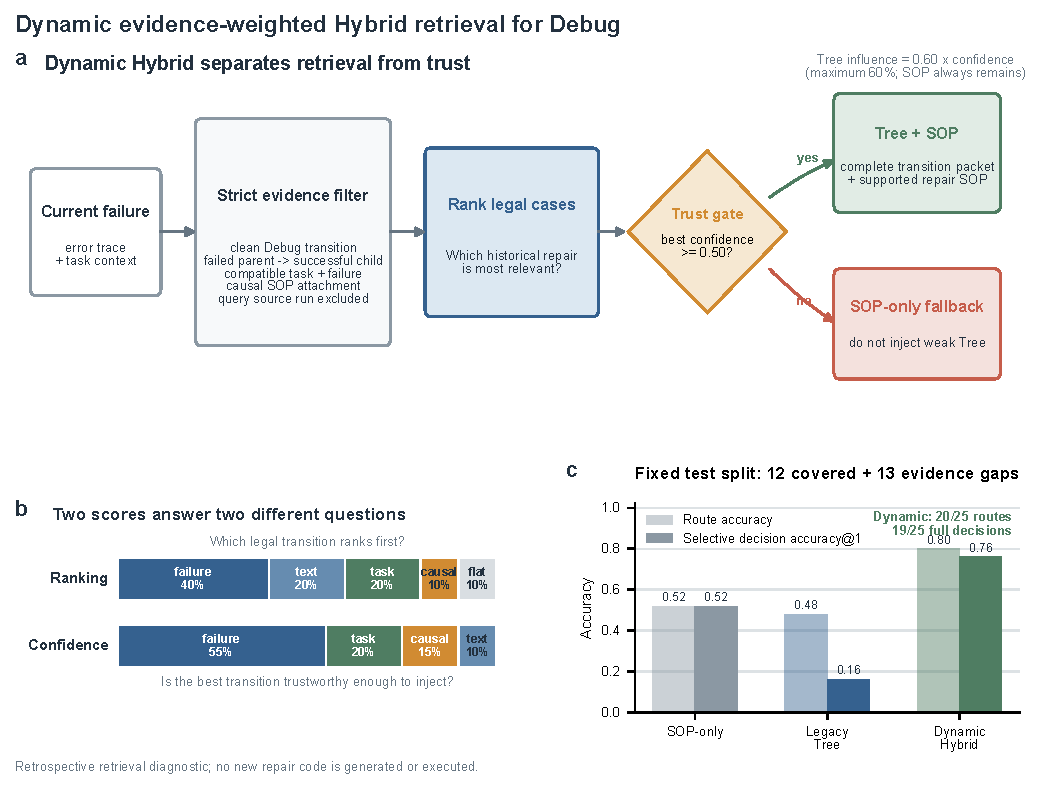
\includegraphics[width=\textwidth]{figures/dynamic_hybrid_explainer.pdf}
  \caption{Dynamic evidence-weighted Hybrid retrieval for Debug.  \textbf{a:}
  The router filters to clean cross-run causal transitions, ranks the legal
  candidates, and then applies an independent trust gate.  Low confidence
  triggers SOP-only fallback; otherwise Tree influence grows with confidence
  but is capped at 60\%.  \textbf{b:} Ranking selects the most relevant legal
  transition, whereas confidence determines whether Tree evidence is admitted.
  \textbf{c:} On the fixed 25-episode retrospective test partition, dynamic
  routing improves route accuracy from 0.48 for legacy Tree to 0.80 and
  Selective Decision Accuracy@1 from 0.16 to 0.76.  No new repair code is
  generated or executed.}
  \label{fig:dynamic-hybrid}
\end{figure*}

\subsection{Method-preserving staged protocol repair}

Programs with potentially valuable methods but invalid evaluation protocols are
not sent to ordinary Improve/Debug.  A deterministic profile selects the needed
repair stages.  For example, early stopping adds validation provenance;
ensembles and supervised second-level features add cross-fitting; learned
weights add selection freeze.  Figure~\ref{fig:repair} shows the maximal path.

\begin{figure*}[t]
  \centering
  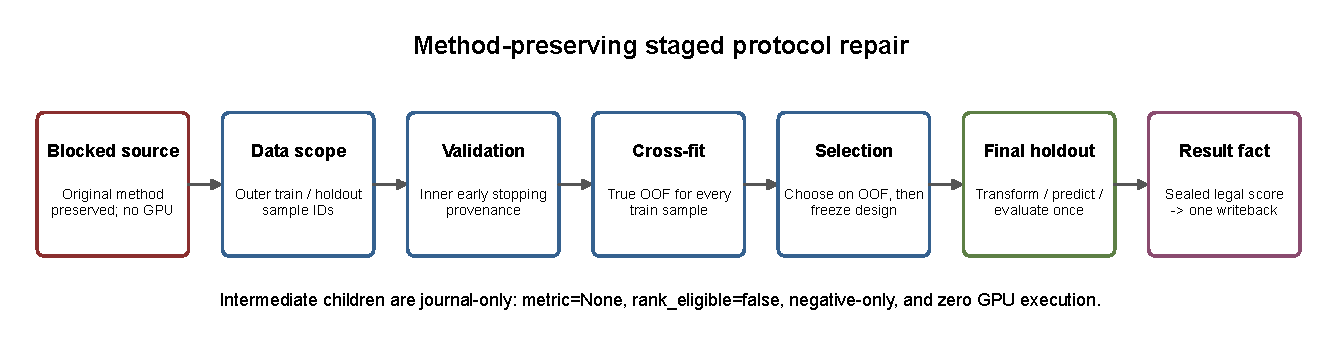
\includegraphics[width=\textwidth]{figures/repair_pipeline.pdf}
  \caption{A maximal staged repair transaction.  The exact path is
  capability-conditioned rather than task- or model-specific.  Intermediate
  children are auditable journal entries but cannot execute, rank, or enter
  positive memory.}
  \label{fig:repair}
\end{figure*}

The preservation contract is extracted once from the source and freezes the
backbone, model and ensemble members, feature families, checkpoint, loss,
optimizer, batch size, epochs, and training budget.  Each stage may alter only
protocol-bearing code such as sample IDs, partitions, fit/transform scopes,
early-stopping splits, OOF assembly, selection scope, and reporting.

The full contract is:

\begin{description}[leftmargin=2.5cm,style=nextline,itemsep=1pt]
  \item[Data scope.] Establish disjoint outer train and holdout IDs; learned
  preprocessing fits inside outer/fold train only.
  \item[Validation provenance.] Ensure early-stopping labels are not used to
  train the corresponding model and remain distinct from final reporting.
  \item[Cross-fit.] Generate every outer-train row's prediction from a model
  that did not train on that row; record exactly-once global OOF coverage.
  \item[Selection freeze.] Select weights, thresholds, or model choices using
  OOF evidence, then freeze all selection state.
  \item[Final holdout.] After freezing, transform, predict, and evaluate the
  outer holdout once.
\end{description}

Rejection reasons and execution tracebacks are injected into the next repair
prompt.  Stage indices and retries are separate: passing one stage advances the
transaction, while bounded retries remain local to the failed stage.

\subsection{Runtime provenance and result publication}

Static analysis cannot prove that runtime arrays match their declared roles.
Generated final candidates use a \texttt{ProtocolProvenanceGuard} to record
partitions, learned-component fit scopes, per-fold predictions, global OOF
coverage, selection scope, freeze time, and final evaluation.  Runtime audit
checks disjointness, OOF exclusion, fit/selection scope, freeze-before-holdout,
and exactly one final evaluation.

The generated guard validates agent-registered events and is not by itself a
proof of all library calls.  The Decision Admissibility layer therefore adds a
separate host-collector boundary for execution, split, fit, prediction,
evaluation, selection, and actuation events.  Production emitter coverage is
still incomplete, but Agent payloads cannot mint a trusted Receipt merely by
claiming \texttt{verified=true}.  Without a clean record, a node cannot become
\texttt{staged\_protocol\_repair\_executed\_clean}, update best artifacts, or
publish a Result Fact.  This code-execution path is distinct from actuation:
the former establishes that the current training artifact ran legally, whereas
the latter establishes that a particular injected historical clause was
realized by that artifact.

\subsection{Experience contracts and versioned writeback}

An admitted clause is compiled into an Experience Contract describing the
expected action or code change.  The system distinguishes exposure, static AST
overlap, runtime activation, counterfactual influence, and legal downstream
outcome.  Three writeback objects prevent two different facts from being hidden
behind one \textsc{Promote} bit.  A \emph{Result Fact} stores the current
artifact, code hash, protocol, score Claim, and authority decision after its own
clean execution.  An \emph{Adoption Edge} additionally requires contract-bound
static and runtime actuation; a \emph{Causal Edge} additionally requires a
paired counterfactual.  Failure to certify an Adoption Edge therefore removes
only the derived-from assertion, not an independently valid Result Fact.

Positive distillation follows the same boundary.  A Positive Result SOP may
summarize a current successful node from its Result Fact and derivation Receipt,
without historical actuation.  A Positive Adopted SOP may say that a historical
experience was realized only when the matching Adoption Edge exists; language
claiming that it caused an improvement additionally requires a Causal Edge.
Retrieval or Agent self-report alone is insufficient for either edge.

Runtime memory is a hash-verified read-only Base Bundle plus an append-only
Session Overlay.  At sleep time, the system audits and decomposes new records,
validates derivation non-escalation, builds a staged child bundle, verifies every
artifact hash, and atomically advances a \texttt{CURRENT} pointer.  Crashes
before publication leave the old Bundle active.  Rollback changes the pointer
without deleting either Bundle or the ledger.

\subsection{Clean Replay creates a new evidence path}

Protocol drift or repairable audit findings may require replay, but historical
Claims are immutable.  A deterministic queue binds task, source run, lineage,
code hash, method hypothesis, method family, and audit disposition.  A
\texttt{MethodFingerprint} protects model and feature families, loss, search
space, compute budget, inference, and ensemble structure while allowing only
ProtocolSpec-declared split, fit, selection, evaluator, and provenance changes.
A preserved method produces a new replay Claim and trusted support path; a
method-changing repair produces a distinct Successor Claim; an unclassified
repair produces neither.  No outcome upgrades the predecessor Claim in place.

\section{Experimental Setup}

We report six different evidence units and do not combine them into one
headline score.

\paragraph{Deterministic authority invariants.}
Unit and integration tests construct mixed-value Claims, forged Receipts,
stale decisions, visibility/cache bypasses, derived-memory laundering,
method-changing replay, concurrent publication, and rollback failures.  These
are executable correctness checks, not estimates of downstream utility.

\paragraph{Split-isolated bundle construction.}
A separate non-Spooky corpus build fingerprints immutable source runs, produces
per-code-node audit sidecars, distills and binds SOP clauses, and publishes Full,
seed-heldout, and task-heldout raw-audited bundles.  The heldout dimensions must
have zero overlap and zero references in the corresponding source Bundle.

\paragraph{Run-tree structural diagnostics.}
These tests ask whether known parent, local-best, neighbor, and failure-recovery
relations are preserved.  They compare Poincar\'e distance, Euclidean distance
on identical coordinates (Flat-Twin), independent Euclidean text features, and
explicit graph expansion.  They measure carrier behavior, not generated-code
quality.

\paragraph{Stage-granularity routing.}
We construct 120 decision episodes spanning Draft, model design, Improve, and
Debug.  Each episode specifies the admissible memory level.  We compare ungated
flat retrieval, Tree-only, SOP-only, and the dynamic stage hybrid using
Granularity Precision@5, Detail Intrusion@5, and empty-result rate.  This track
tests whether the abstraction gate returns the right kind of memory; it does not
test whether generated code improves a task metric.

\paragraph{Causal Debug transfer.}
We derive 38 real Debug episodes from 12 source-run journals and use a fixed
source-run partition of 13 development and 25 test episodes.  A covered episode
has at least one compatible successful transition from another run; a coverage
gap has none.  The test split contains 12 covered episodes and 13 gaps.  Systems
compare SOP-only fallback, random transition, task-only transition, lexical
transition, legacy successful-node Tree retrieval, and the dynamic causal
hybrid.  Route accuracy rewards selecting Tree only when evidence exists;
Selective Decision Accuracy@1 rewards either retrieving a correct transition on
covered episodes or correctly falling back on gaps.  Each covered episode can
have multiple silver-gold transitions.  Per-episode Hit@1 is one when the first
result is in that set; Recall@5 is the fraction of that set recovered in the
first five; and MRR is the reciprocal rank of the first matching transition.
We macro-average these quantities over covered episodes.  Candidate filtering
excludes the query source run and unsafe evidence by construction.

The benchmark is retrospective: the graph was visible during system development,
the fixed test partition is not a blind held-out study, and deterministic failure
labels are produced by a separate code path but are semantically aligned silver
labels.  It therefore supports a routing diagnostic, not a generalization or
downstream-execution claim.

\paragraph{Prospective dual-observer prevalence audit.}
We run four natural MLE tasks (Denoising, Leaf, Aerial, and Taxi) with three
agent seeds each, yielding 12 run packets whose online packet gates are
verified.  At every decision opportunity, the observer records the retrieval
system's \texttt{raw\_candidate\_ids} before Authority, the gate's
\texttt{suppressed\_candidate\_ids}, and the
\texttt{final\_prompt\_candidate\_ids} after enforcement.  Thus the actual
agent remains protected while the raw proposal distribution remains auditable.
A known-invalid Spooky experience is planted as a positive control and is
reported separately from natural rates.  A partially completed run contributes
only when its packet gate and completed decision ledger are verified; it is not
treated as an 80-step performance result.  The primary endpoint is automatic
candidate-level suppression, not Oracle-adjudicated invalid prevalence.

\paragraph{Preregistered same-domain online evaluation.}
After the failed first shadow attempt was retained as an infrastructure-abort
artifact, a corrected WP7 shadow/canary gate and the WP8 staging gate were
completed.  The formal Tier-2 design used three same-domain target tasks
(image, audio, and tabular), three agent seeds, five online systems per block,
and one host-only Oracle disposition per block.  The sample unit is the assigned
task--seed--system condition.  Host-owned terminal evaluators produced 22
protocol-legal selected scores; all 23 failures remained outcomes with no score
imputation or post-assignment exclusion.  Source-task scores and target-task
history were never inherited.  Historical values 0.2013 and 0.0494 remain
excluded (Section~\ref{sec:failure}).

\paragraph{Sequential Spooky memory-accumulation case study.}
We additionally trace one authorship-attribution task through a clean no-memory
cold start, a one-run memory package, a two-run memory package, and a final
all-history package.  At each stage we report one audit-qualified, externally scored
submission and retain both Kaggle public and private multiclass log-loss.  The
final package admits 56 historical journals, while static audit and typed
distillation keep clean, blocked, and warning evidence distinct.  Because the
four stages differ in historical coverage, replay target, and implementation
state and contain one selected run each, this is a sequential case study rather
than a randomized memory-on/off effect estimate.

\paragraph{Cross-task Leaf-to-Plant tournament case study.}
We evaluate one transfer from a frozen Leaf memory snapshot to Plant Seedlings.
The snapshot registers 96 historical source runs; four independently retrieved
seats are then constructed from Leaf evidence.  The terminal attempt uses one
NVIDIA A100 80~GB GPU, 8 CPU cores, 32~GiB memory, one worker,
GPT-5.6-sol at low reasoning effort, and a 21,600-s search budget.  Public
pretrained assets are allowed by the target execution contract.  We retain all
seven independent no-memory Novel runs with official scores as a descriptive
reference set.  These runs are heterogeneous in model access, pretrained-asset
access, compute, CPU allocation, and framework version.  Transfer records are
restricted to tournament-era attempts 001--005, all of which have official
score ledgers.  Run status is reported separately from official-score status;
attempt 005 is the only terminal-complete search.

\paragraph{Cross-task Spooky-to-Detecting-Insults search case study.}
We compare five strict no-memory Novel searches on Detecting Insults with five
searches that retrieve from a frozen all-history Spooky Author Identification
memory package.  A plotted point is an internal validation ROC--AUC from a
numeric, valid, non-buggy, rank-eligible candidate.  Protocol-biased candidates
are removed before computing the running maximum.  The horizontal coordinate
is the original global journal step, so a blank prefix means that no admissible
score has yet been produced; it is not backfilled at step zero.  We report the
candidate-score median and interquartile range (IQR), the distribution of the
five final running-best values per condition, and the first admissible-score
step.  For an interpretable early-stopping diagnostic, we also use ROC--AUC
0.93 as a descriptive viable-candidate threshold; it was not preregistered.
The runs differ in execution environment, model access, and trajectory length.
Per-step GPU time and LLM-token receipts are not harmonized, so steps to
threshold are a budget proxy rather than a measured cost ratio.

\section{Results}

\subsection{The authority boundary is active in natural decision streams}
\label{sec:prospective-prevalence}

Across the 12 verified natural run packets, the prospective observer records
171 decision opportunities and 4,106 raw historical-memory candidates.  The
Authority Gate automatically suppresses 783 candidates before final prompt
construction, a candidate-level suppression rate of 19.07\%.  At least one
candidate is suppressed in 169/171 decisions (98.83\%).  The latter is an
opportunity-level activation statistic---each decision contains multiple
candidates---and must not be read as the fraction of memories that are invalid.
Table~\ref{tab:prospective-prevalence} reports the natural-task breakdown.

\begin{table}[t]
\caption{Prospective dual-observer audit over verified natural run packets.
``Suppressed'' means automatically removed by the Authority Gate before final
Prompt construction; it does not mean independently adjudicated invalid.}
\label{tab:prospective-prevalence}
\centering
\small
\begin{tabular}{lrrrr}
\toprule
Task & Decisions & Raw & Suppressed & Rate \\
\midrule
Denoising & 35 & 824 & 188 & 22.82\% \\
Leaf      & 39 & 1,116 & 171 & 15.32\% \\
Aerial    & 32 & 765 & 130 & 16.99\% \\
Taxi      & 65 & 1,401 & 294 & 20.99\% \\
\midrule
Total     & 171 & 4,106 & 783 & 19.07\% \\
\bottomrule
\end{tabular}
\end{table}

In the separately reported positive-control packet, the known-invalid
experience appears once in the raw candidate set and has zero actual Prompt
exposures.  This establishes that the observer records a pre-gate opportunity
that enforcement can block at the real Prompt boundary.  It does not establish
the precision or recall of suppression on natural candidates: those quantities
require independent candidate-level Oracle labels.

\subsection{Claim-level visibility preserves useful parts of mixed experience}

A deterministic mixed-value SOP contains three clauses: a valid
sample-ID-based OOF alignment repair, an audit warning that the historical
selection read report labels, and the resulting contaminated score.  Under
Debug, the repair and warning remain visible while the score is suppressed.
Under Rank, the pack is empty: the score clause is absent from embedding and
RRF candidates, absent from the prompt, and consumes zero tokens.  The test
therefore obtains $2/2$ oracle-legal Debug clause retention, zero unauthorized
prompt exposure, and zero unauthorized activation.

The bypass controls attempt to reintroduce denied content through quarantined
navigation edges, legacy \texttt{distills\_to}, forged
\texttt{attached\_sop\_ids}, Tree projection, and stale cached decisions.  All
are suppressed; only an explicitly authorized adoption edge is consumable.
On the frozen legacy graph, 281 SOP containers materialize to 843 clauses and
2,773 warning-only navigation edges.  Inspect and Debug can retain those clauses
as warnings, whereas Rank consumes zero of the 2,773 edges.  These are exact
invariant checks, not a prevalence or task-performance estimate.

\subsection{Separated writeback preserves independent success without inventing ancestry}

The deterministic writeback fixture starts with a clean current node that has
not been exposed to any historical experience.  \textsc{Promote-Result}
publishes exactly one Result Fact with an empty \texttt{derived\_from} field.
After one source Claim is injected and its contract reaches static/runtime L3,
\textsc{Publish-Adoption} appends exactly one Adoption Edge.  The same contract
cannot publish a Causal Edge until a valid memory-on/off pair reaches L4; after
that condition, exactly one Causal Edge is appended.  Repeated calls are
idempotent, and the Bundle publisher inventories all three objects separately.

Two adjacent fixtures close the lifecycle.  Fixed-holdout search writes no
positive memory before terminal scoring; the sealed scorer then writes exactly
one Result Fact, while tampering produces an explicit incomplete status and no
partial result.  Positive Result SOP distillation succeeds from the target
node's own legal evidence without historical actuation, whereas Positive
Adopted SOP distillation is denied until the matching contract reaches L3 and
causal wording additionally requires L4.  These are deterministic software
invariants, not estimates of adoption prevalence or downstream benefit.

\subsection{Real-corpus bundles preserve split and authority boundaries}

The formal non-Spooky build inventories 90 directories: 79 complete runs across
16 tasks and 11 incomplete directories excluded from every split.  All 1,577
code nodes receive an immutable audit sidecar; no source journal is modified.
Table~\ref{tab:bundle} reports the main artifacts.  The binder emits 1,545
clauses with resolvable sources and no scope widening.  Compilation conservatively
downgrades 513 proposed publication classes and emits zero certified clauses,
which is required for a raw-audited rather than replay-certified Bundle.

\begin{table}[t]
\caption{Decision Admissibility corpus and bundle evidence.  Counts describe
the separate non-Spooky formal build, not the older routing benchmark graph.}
\label{tab:bundle}
\centering
\small
\begin{tabular}{lr}
\toprule
Artifact or disposition & Count \\
\midrule
Complete runs / tasks & 79 / 16 \\
Run nodes / code nodes & 1,656 / 1,577 \\
Scored metric nodes & 589 \\
Audit: clean / warning & 718 / 40 \\
Audit: blocked / unavailable & 655 / 164 \\
Bound clauses / merged containers & 1,545 / 934 \\
Diagnostic / candidate / certified clauses & 1,278 / 267 / 0 \\
\bottomrule
\end{tabular}
\end{table}

The seed-heldout Bundle contains 53 source and 26 heldout runs with zero run or
seed-group overlap.  The task-heldout Bundle contains 58 source and 21 heldout
runs, corresponding to 12 source and four heldout tasks with zero task/run
overlap and zero heldout references.  All three published raw-audited Bundles
have zero authorized adoption edges and pass external hash validation.  This
establishes corpus isolation and publication integrity, not model
generalization.

\subsection{Stratification removes cross-level detail intrusion}

Table~\ref{tab:granularity} and Figure~\ref{fig:retrieval}A report the
stage-granularity track.  The ungated retriever mixes memory levels: only 0.4467
of its top-five items have the requested granularity and 0.5533 are intrusions.
Both SOP-only and the dynamic hybrid achieve 1.0000 precision with zero
intrusion, while Tree-only is precise when it answers but returns an empty result
on 24.17\% of episodes.  The result verifies the deterministic abstraction gate
over these episodes; equal SOP-only precision also shows that this track alone
cannot establish the value of causal Tree evidence.

\begin{table}[t]
\caption{Stage-granularity routing over 120 retrospective episodes.}
\label{tab:granularity}
\centering
\small
\begin{tabular}{lrrr}
\toprule
System & Granularity P@5 $\uparrow$ & Intrusion@5 $\downarrow$ & Empty $\downarrow$ \\
\midrule
Ungated flat & 0.4467 & 0.5533 & 0.0000 \\
Tree-only & 0.7583 & \textbf{0.0000} & 0.2417 \\
SOP-only & \textbf{1.0000} & \textbf{0.0000} & \textbf{0.0000} \\
Dynamic stage hybrid & \textbf{1.0000} & \textbf{0.0000} & \textbf{0.0000} \\
\bottomrule
\end{tabular}
\end{table}

\begin{figure*}[t]
  \centering
  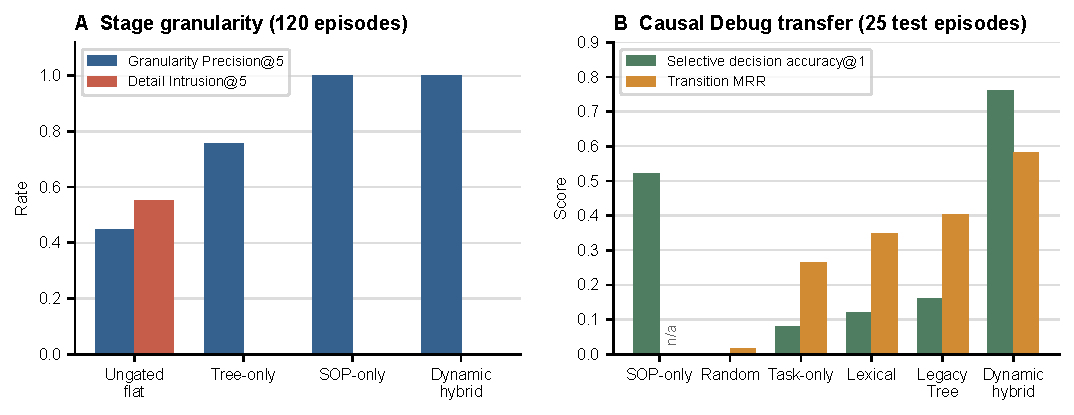
\includegraphics[width=\textwidth]{figures/retrieval_results.pdf}
  \caption{Retrospective routing diagnostics.  \textbf{A:} Stage stratification
  removes cross-level detail intrusion over 120 episodes.  \textbf{B:} On the
  fixed 25-episode causal Debug test partition (12 covered, 13 gaps), the dynamic
  hybrid improves both evidence routing and transition recovery.  SOP-only has
  no transition MRR because it cannot return a Tree transition.  The benchmark
  uses semantically aligned silver labels and does not execute new repairs.}
  \label{fig:retrieval}
\end{figure*}

\subsection{Failure-matched causal transitions improve Debug decisions}

Table~\ref{tab:causal} and Figure~\ref{fig:retrieval}B report the fixed causal
Debug test partition.  Legacy Tree retrieval selects Tree for every covered
episode but cannot recognize gaps, yielding 0.4800 route accuracy and 0.1600
Selective Decision Accuracy@1.  Random, task-only, and lexical controls show
that source-run exclusion and broad compatibility are insufficient.  The
dynamic hybrid matches the failure mechanism, ranks complete transitions, and
falls back when evidence is weak.  It reaches 0.8000 route accuracy, 0.7600
selective decision accuracy, and 0.5833 transition MRR.  Relative to legacy
Tree, the gains are $+0.3200$, $+0.6000$, and $+0.1806$, respectively.

The episode counts make the operational difference explicit.  SOP-only always
abstains: it is correct on all 13 evidence gaps but cannot solve any of the 12
covered episodes, giving $13/25=0.52$ selective accuracy.  Legacy Tree fails to
abstain on gaps and retrieves a correct top-ranked transition in only four
covered episodes, giving $4/25=0.16$.  The dynamic route chooses Tree correctly
for eight covered episodes, retrieves the correct top transition for seven, and
falls back on 12 of 13 gaps.  It therefore obtains $20/25=0.80$ route accuracy
and $(7+12)/25=0.76$ selective accuracy.  Its advantage is selective use of
specific evidence, not uniformly greater reliance on Tree memory.

\begin{table}[t]
\caption{Causal Debug retrieval on the fixed 25-episode test partition.  Hit@1
and MRR are defined on the 12 covered episodes; fallback is defined on 13 gaps.}
\label{tab:causal}
\centering
\footnotesize
\begin{tabular}{lrrrrr}
\toprule
System & Route & Selective@1 & Hit@1 & MRR & Fallback \\
\midrule
SOP-only & 0.5200 & 0.5200 & n/a & n/a & 1.0000 \\
Random transition & 0.4800 & 0.0000 & 0.0000 & 0.0167 & 0.0000 \\
Task-only transition & 0.4800 & 0.0800 & 0.1667 & 0.2639 & 0.0000 \\
Lexical transition & 0.4800 & 0.1200 & 0.2500 & 0.3472 & 0.0000 \\
Legacy success Tree & 0.4800 & 0.1600 & 0.3333 & 0.4028 & 0.0000 \\
Dynamic causal hybrid & \textbf{0.8000} & \textbf{0.7600} & \textbf{0.5833} & \textbf{0.5833} & 0.9231 \\
\bottomrule
\end{tabular}
\end{table}

All compared methods produce zero unsafe-candidate and query-source-run escapes,
because these are enforced candidate-filtering invariants rather than empirical
safety discoveries.  The diagnostic gain is therefore narrower: among legal
candidates, the dynamic route more often chooses whether Tree evidence is
appropriate and which historical transition matches the current failure.

\subsection{Static audit substantially changes evidence eligibility}

Table~\ref{tab:audit} shows the V3 status distribution over 1,324 code-bearing
RunNodes.  Only clean nodes may support certified ranking.  The audit broadens
holdout-alias and arbitrary fit-receiver coverage while treating train-only
pre-CV fitting as warning-level protocol evidence.  The claim is intentionally
limited: exact and normalized-structure matches can block known leaked code;
semantic similarity is advisory to avoid an uncontrolled false-positive
surface.

\begin{table}[t]
\caption{Static audit status over code-bearing RunNodes.}
\label{tab:audit}
\centering
\small
\begin{tabular}{lrr}
\toprule
Status & Count & Positive/rank eligible? \\
\midrule
Clean & 693 & potentially, after execution checks \\
Blocked & 280 & no \\
Protocol-biased & 55 & no; staged repair only \\
Warning & 155 & no certified promotion \\
Audit unavailable & 141 & no (fail closed) \\
\bottomrule
\end{tabular}
\end{table}

\subsection{Replay recovery and publication pass deterministic invariants}

The focused Clean Replay suite covers deterministic queue selection, exact raw
code/lineage binding, method preservation, method-changing fake repair,
cross-artifact Receipt rejection, new-Claim recovery, immutable child-Bundle
publication, and runtime reload.  A method-preserved replay authorizes only its
new clean Claim; a model, feature, loss, search-space, budget, inference, or
ensemble change produces a Successor Claim; the predecessor and unrelated
historical scores remain denied.  Crash-safe publication and rollback tests
retain both Bundles and the append-only ledger.

The final host regression binds seven green runs and 1,454 executed tests with
zero failures, errors, or skips; the full suite contributes 760 tests and the
frozen composite module contributes 19.  A 579-entry source/test-dependency
inventory is byte-identical before and after execution.  Two historical
failure-to-fix chains are retained rather than overwritten.  The corrected WP7
shadow/canary, Tier-0, controlled Tier-1, and multi-generation gates all pass;
these engineering and mechanism results do not override the formal effect
gate.

\subsection{Formal same-domain transfer does not establish superiority}
\label{sec:formal-online}

The formal intention-to-treat population contains nine task--seed blocks, 45
assigned online conditions, and nine host-only Oracle dispositions.  Full,
Flat Relevance Memory, Global Validity Bit, and Authority Only each complete
4/9 conditions; No Memory completes 6/9.  Every successful condition emits one
independent Result Fact and every failed condition emits none.  No assignment is
imputed or excluded after assignment.

\begin{table}[t]
\caption{Preregistered Full-minus-No-Memory result.  Continuous comparisons use
only blocks where both systems produced protocol-legal selected scores; failures
remain in the intention-to-treat completion denominator.}
\label{tab:formal-online}
\centering
\small
\begin{tabular}{lr}
\toprule
Quantity & Result \\
\midrule
Assigned task--seed pairs & 9 \\
Full / No Memory completed & 4 / 6 \\
Both scored / unavailable & 4 / 5 \\
Available-pair wins / ties / losses & 4 / 0 / 0 \\
Exact one-sided sign-flip $p$ & 0.0625 \\
Holm-adjusted $p$ & 0.25 \\
Taxi scored pairs & 0 \\
Task-macro bootstrap & not estimable \\
Frozen superiority gate & rejected \\
\bottomrule
\end{tabular}
\end{table}

Among the four score-estimable pairs, the mean Full-minus-No-Memory macro-F1
difference is $+0.014373$ on Aerial Cactus (three pairs) and $+0.059794$ on
Birds (one pair).  This is an available-pair diagnostic, not a population trend:
five assigned pairs are unavailable, Full has two more completion failures than
No Memory, and Taxi contributes no estimable pair.  The frozen effect gate fails
six of eight criteria.  The Evidence Ledger therefore marks Full superiority
\emph{rejected}, conditional utility \emph{diagnostic}, and experience causality
\emph{pending}.  The formal system contrast is not an L4 memory-on/off receipt.

The first four completed blocks bind source snapshot \texttt{d7fed754...}; the
five result-blind retry blocks bind \texttt{c674364d...}.  The r9 amendment,
frozen before result analysis, attests that the difference is restricted to
schema and receipt plumbing and changes no candidate-generation, retrieval,
condition, evaluation, or writeback semantics.  Post-result safety fixes are
tested only in the closeout regression and are not credited to the formal
effect estimate.

\subsection{Audited accumulated memory improves the final Spooky replay, but the trajectory is non-monotone}
\label{sec:spooky-iterative-memory}

Figure~\ref{fig:spooky-iterative-memory} follows the Spooky Author
Identification task from a clean no-memory reproduction through two bounded
memory iterations and a final all-history replay.  The clean cold start obtains
public/private log-loss 0.34318/0.32388.  One-run memory improves this to
0.31505/0.30095, whereas the two-run exact replay slightly regresses to
0.33494/0.30940.  Thus the intermediate observations do not support a monotone
``more memory is better'' claim.

The final package expands to 56 historical journals and 1,914 run nodes, but it
does not expose all history as positive guidance: 730 audited code nodes are
clean, 638 are blocked, and the package contains 1,681 evidence items and 22
stratified SOPs.  After the isolation audit, retrieval smoke test, and clean
DeBERTa replay binding pass, the selected replay reaches public/private
log-loss 0.27986/0.25613.  Relative to the clean cold start, private log-loss is
lower by 0.06775 (20.9\%).  This result is consistent with useful accumulated
memory only when evidence admission and replay actuation are both enforced; it
does not isolate memory quantity from the replay fix or establish an L4 causal
edge.

\begin{figure*}[t]
  \centering
  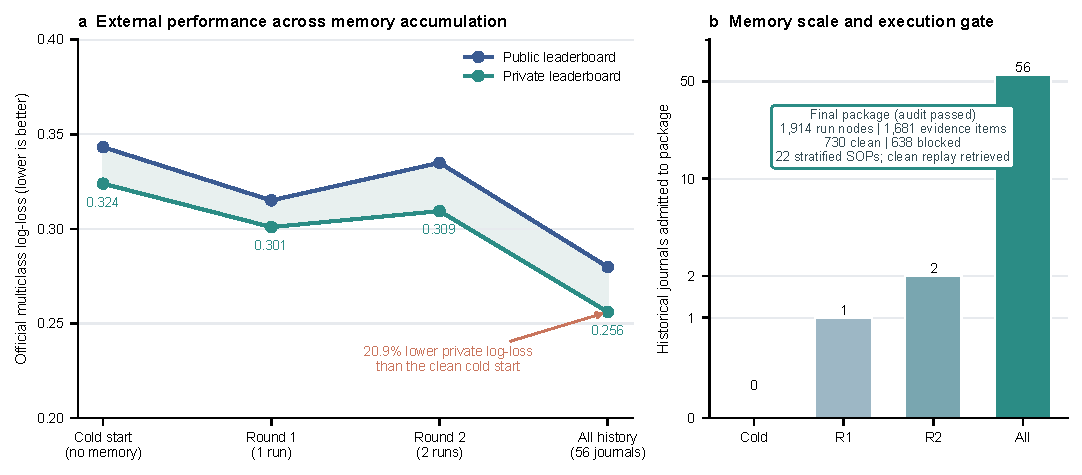
\includegraphics[width=\textwidth]{figures/spooky_iterative_memory.pdf}
  \caption{Sequential Spooky memory-accumulation case study.  \textbf{a:}
  Kaggle public and private multiclass log-loss for one selected submission at
  each stage (lower is better), shown on a shared 0.20--0.40 axis so the small
  second-to-third-stage regression is not visually magnified.  The two bounded
  memory rounds are non-monotone, while the audited all-history replay gives
  the strongest external score.
  \textbf{b:} Historical-journal count in each memory package and the audited
  composition of the final package.  Points are single runs without uncertainty
  intervals.  The comparison is descriptive because memory coverage, selected
  replay target, and implementation state change together.}
  \label{fig:spooky-iterative-memory}
\end{figure*}

\subsection{Leaf memory transfer reaches the upper end of the Plant reference range}
\label{sec:leaf-plant-transfer}

Across seven independent no-memory Novel searches, official scores range from
0.76574 to 0.98362, with median 0.93450.  The five tournament attempts have
official scores from 0.97355 to 0.98236.  Attempt 002 is the best at 0.98236:
it exceeds six of the seven observed Novel runs and is 0.00126 below the
unrestricted v159 result (0.98362).  Thus the official transfer results occupy
the upper end of the observed reference range, but are not uniformly best
(Figure~\ref{fig:leaf-plant-transfer}).

Attempts 001 and 003 score 0.97355 and 0.97481, respectively; they stopped at a
finalization-reserve defect and a donor-queue deadlock.  Attempts 002 and 004
score 0.98236 and 0.97607; attempt 002 was censored during baseline
qualification, and attempt 004 failed terminal finalization without a frozen
champion.  These are valid external scores, while their run-status limitations
remain explicit.  Because the historical Novel controls are not
configuration-matched, this case study does not identify a causal effect of
transferred memory.

\FloatBarrier
\begin{figure*}[t]
  \centering
  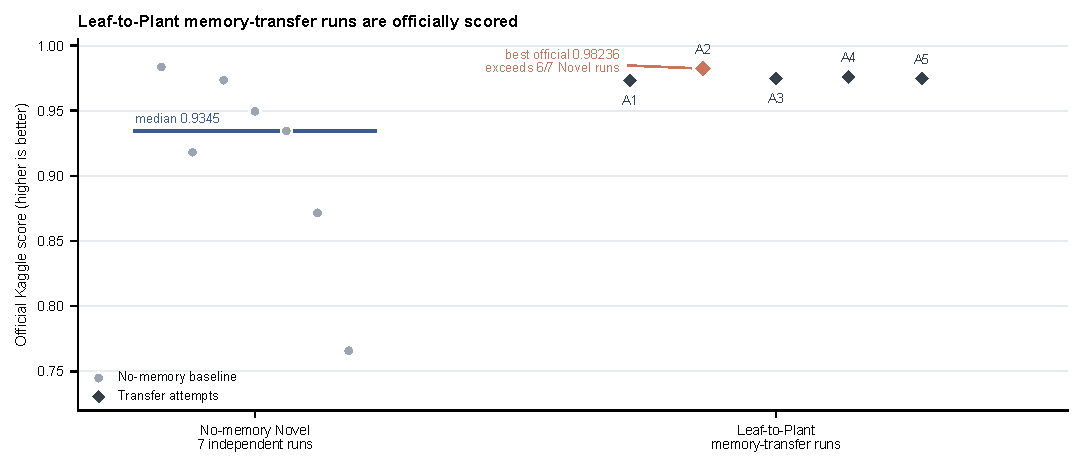
\includegraphics[width=\textwidth]{figures/plant_leaf_transfer_tournament.pdf}
  \caption{Cross-task Leaf-to-Plant transfer after tournament activation.
  Official Plant Seedlings scores for all seven independent
  no-memory Novel runs and all five tournament-era transfer attempts.  Circles
  denote no-memory baselines and diamonds denote transfer attempts; all marks
  have complete Kaggle score ledgers.  The blue horizontal segment marks the
  Novel median, and the orange diamond highlights the highest transfer score.
  Each mark is one officially scored run; no uncertainty interval is implied.
  The comparison is descriptive because execution contracts differ across the
  historical controls.}
  \label{fig:leaf-plant-transfer}
\end{figure*}

\subsection{Spooky memory transfer concentrates strong Detecting Insults candidates early}
\label{sec:detecting-insults-transfer}

The first rank-eligible score appears at median global step 2 under transfer
(range 1--3), compared with step 4 for Novel search (range 1--48).  All five
transfer runs produce a valid score by step 3, whereas only two of five Novel
runs do so.  At the descriptive ROC--AUC 0.93 threshold, every transfer run
crosses by step 3.  Only three Novel runs ever cross, at steps 1, 4, and 5; the
other two remain below 0.93 through terminal steps 44 and 137
(Figure~\ref{fig:detecting-insults-search}).

The retained score distributions show the same concentration.  Across 59
transfer candidate points, the median ROC--AUC is 0.9305 (IQR 0.0255), compared
with 0.9212 (IQR 0.0414) across 121 Novel points.  Across the five final
running-best values per condition, transfer has median 0.9533 and IQR 0.0105;
Novel has median 0.9417 and IQR 0.0589.  Thus the transferred runs produce
earlier viable candidates, a tighter candidate distribution, and substantially
less dispersion in final best scores.

This shift is operationally useful.  Under an early-stop rule at ROC--AUC 0.93,
all five transfer searches could stop by step 3, while two Novel searches would
continue spending search budget without reaching the threshold.  Under
comparable per-step costs, fewer pre-threshold steps imply lower GPU occupancy
and fewer LLM-guided proposal and review calls.  The experiment does not log a
configuration-matched token or GPU-hour counterfactual, however, so it supports
lower budget demand as a search-efficiency implication, not a measured cost
reduction or a causal memory-effect estimate.  Candidate points within a run
are also dependent; the point-level summaries are descriptive and no
candidate-level significance test is applied.

\FloatBarrier
\begin{figure*}[t]
  \centering
  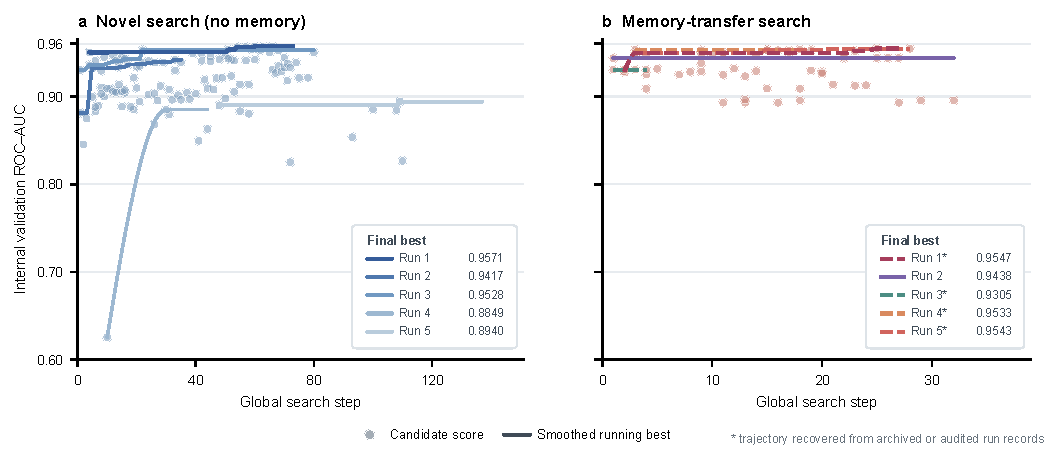
\includegraphics[width=\textwidth]{figures/detecting_insults_search_curves.pdf}
  \caption{Spooky-to-Detecting-Insults search trajectories.  \textbf{a:}
  Five strict no-memory Novel searches.  \textbf{b:} Five searches using the
  transferred Spooky memory package.  Dots are retained candidate internal
  validation ROC--AUC values; lines are shape-preserving interpolations of the
  observed running maximum.  Both panels use the same vertical scale.  Global
  search step is the original journal index, and each line begins at its first
  rank-eligible scored candidate; empty prefixes therefore mean ``no admissible
  score yet.''  Asterisks identify trajectories recovered from archived or
  audited run records.  Each panel contains five search runs without
  uncertainty intervals.  Execution contracts and validation partitions are
  not fully matched, so the comparison is descriptive.  Source data are
  provided with the paper artifacts.}
  \label{fig:detecting-insults-search}
\end{figure*}

% Multi-round memory accumulation on two agent harnesses (results as of 2026-09-22).
% Figures are the current working (Chinese-labelled) exports; they will be redrawn
% in English before submission.  Source CSVs and plotting scripts are in the
% GitHub paper branch under results/multiround_20260922/.

\subsection{Multi-round memory accumulation on two agent harnesses}
\label{sec:multiround-two-harness}

To test whether distilled cross-round memory is useful outside one agent
implementation, we repeat the round-by-round protocol on two harnesses.
\textbf{MLEvolve} is the multi-agent search harness used in the rest of this
paper (planner, coder, reviewer, and an inner AgentTuner, with the frozen v7
runtime).  \textbf{autoresearch} is a port of a single-agent research loop:
one agent edits a candidate training script, the host executes it and keeps or
discards it; there is no MLEvolve searcher, reviewer, or inner agent.  The two
harnesses share only the memory-pack format (search-experience and
inner-tuning cards) and the execution container.

\paragraph{Protocol.}
Round~1 (R1) runs with no memory.  Each later round may read only memory cards
distilled from the earlier rounds listed in Table~\ref{tab:multiround-summary};
it never reads their code, checkpoints, or task packages.  Every round has a
7{,}200\,s budget and a 3{,}600\,s per-node cap, a single seed, and one fixed
internal split.  ``Host'' scores are recomputed by the host from a validated
checkpoint on a held-back \emph{search} split whose labels the agent never sees;
``tune'' scores are candidate-reported values on the agent-visible tune split.
None of these are Kaggle leaderboard scores, and the search split is used
adaptively across candidates within a run.

\begin{table*}[t]
  \centering
  \caption{Best score per round for the multi-round memory experiments
  (single seed per round; ``$\downarrow$'' lower is better, ``$\uparrow$''
  higher is better).  Memory column lists the rounds whose distilled cards
  were readable.  MLE = MLEvolve; AR = autoresearch.  All values are internal
  Host or tune scores, not Kaggle scores.}
  \label{tab:multiround-summary}
  \small
  \setlength{\tabcolsep}{4pt}
  \begin{tabular}{@{}lllll@{}}
    \toprule
    Harness & Task (metric) & Round & Memory read & Best score \\
    \midrule
    \multirow{5}{*}{MLE} & \multirow{5}{*}{Leaf (Host search log-loss $\downarrow$)}
      & R1 & none & 0.443894 \\
    & & R2 & R1 & 0.442665 \\
    & & R3 & R1+R2 & 0.066774 \\
    & & R5$^\dagger$ & R1--R4 (91 cards) & 0.042636 \\
    & & R6$^\dagger$ & R5 pack (repeat) & 0.035167 \\
    \midrule
    \multirow{4}{*}{MLE} & \multirow{4}{*}{Spooky (Host search log-loss $\downarrow$)}
      & A$^\dagger$ & none & 0.35620 \\
    & & C & A & 0.31031 \\
    & & D & A+B+C & 0.27670 \\
    & & E & A+B+C+D & 0.25928 \\
    \midrule
    \multirow{4}{*}{MLE} & \multirow{4}{*}{iMet 2020 (Host micro-F1 $\uparrow$)}
      & R1 & none & 0.42416 \\
    & & R2 & R1 & 0.50491 \\
    & & R3 & R1+R2 & 0.51130 \\
    & & R4 & R1+R2+R3 & 0.58865 \\
    \midrule
    \multirow{4}{*}{MLE} & \multirow{4}{*}{Plant Pathology 2021 (Host micro-F1 $\uparrow$)}
      & R1 & none & 0.83857 \\
    & & R2 & R1 & 0.85573 \\
    & & R3 & R1+R2 & 0.86316 \\
    & & R4 (repeat) & R1+R2+R3 & 0.86077 \\
    \midrule
    \multirow{3}{*}{AR} & \multirow{3}{*}{iMet 2020 (tune micro-F1 $\uparrow$)}
      & R1 & none & 0.38823 \\
    & & R2 & R1 & 0.43860 \\
    & & R3 & R1+R2 & 0.45849 \\
    \midrule
    \multirow{4}{*}{AR$^\ddagger$} & \multirow{4}{*}{Spooky (Host search log-loss $\downarrow$)}
      & R1 (MLE) & none & 0.35028 \\
    & & R2 & R1 & 0.35111 \\
    & & R3 & R1+R2 & 0.34911 \\
    & & R2 rerun & new AR R1 & 0.35625 \\
    \midrule
    \multirow{3}{*}{AR$^\ddagger$} & \multirow{3}{*}{Leaf (Host search log-loss $\downarrow$)}
      & R1 (MLE) & none & 0.44389 \\
    & & R2 & R1 & 0.06357 \\
    & & R3 (MLE) & R1 + orig.\ MLE R2 & 0.06677 \\
    \bottomrule
  \end{tabular}

  \vspace{2pt}
  {\footnotesize $^\dagger$Part of the budget was resumed after a provider
  outage with a different model, provider, or GPU host.
  $^\ddagger$Mixed series: only the rounds without the ``(MLE)'' tag ran on
  autoresearch; the MLE rounds are the memory sources or reference points.}
\end{table*}

\paragraph{MLEvolve: memory rounds reach better scores on all four tasks.}
On every MLEvolve task, the best memory-enabled round is better than the
no-memory R1 (Table~\ref{tab:multiround-summary}).  On Leaf
(Figure~\ref{fig:mle-leaf-rounds}), R1 and the one-round-memory R2 stay near
0.44 Host log-loss, whereas R3 reaches 0.0668 and the rounds reading the
91-card cumulative pack reach 0.0426 and 0.0352; the first certified R6
candidate already appears at about 13 minutes.  On Spooky
(Figure~\ref{fig:mle-spooky-acde}), Host log-loss decreases with each added
memory source, from 0.3562 (A) to 0.3103 (C), 0.2767 (D), and 0.2593 (E); D's inner-tuning trajectory starts below A's
final tune loss, and E ends with the lowest tune loss (0.2643).  On
iMet (Figure~\ref{fig:mle-imet-rounds}) Host micro-F1 increases from 0.4242 to
0.5049, 0.5113, and 0.5887.  On Plant Pathology
(Figure~\ref{fig:mle-pp21-rounds}) it increases from 0.8386 to 0.8557 and
0.8632; the R4 repeat (0.8608) is slightly below R3, so the gain saturates
after two memory rounds and is not monotone.

\paragraph{autoresearch: the same memory transfers to a single-agent loop.}
The cleanest cross-harness evidence is iMet on autoresearch
(Figure~\ref{fig:ar-imet-rounds}), where model, data split, runtime, and budget
are fixed across rounds.  The calibrated tune micro-F1 rises from 0.3882 (R1)
to 0.4386 (R2) and 0.4585 (R3), and the round best arrives earlier
(89.3, 79.6, and 65.3 minutes).  Host recomputation agrees
(0.3892, 0.4410, 0.4586).  On Leaf (Figure~\ref{fig:ar-leaf-rounds}), an
autoresearch R2 that reads memory distilled from the MLEvolve R1 reaches
0.0636 Host log-loss, compared with 0.4439 for that R1; one of its candidates
reproduces the R1 best exactly (0.443894), indicating that the recipe was
carried over by memory before being improved.  On Spooky
(Figure~\ref{fig:ar-spooky-rounds}) the effect is small: autoresearch R2 and R3
obtain 0.3511 and 0.3491 against 0.3503 for the MLEvolve R1 memory source,
and a rerun of R2 that read a new autoresearch R1 obtains 0.3562 after a
provider failure stopped it at about 60 minutes.

\paragraph{What these results do and do not show.}
These are descriptive single-seed trajectories, not controlled ablations.
Several confounds change together with memory:
(i) the model changes from Luna to Terra in the MLEvolve iMet and Spooky
chains and between harnesses on Leaf;
(ii) some rounds were resumed after provider outages on a different host or
provider (Leaf R5/R6, Spooky A/C, iMet R4), and several runs ended by a
watchdog rather than normally;
(iii) runtime patches were introduced between rounds (for example the iMet
recipe contract from R3 and the Plant Pathology R1 wall-clock versus later
effective-time budgets);
(iv) some series are curated: Leaf R4 and the original Leaf R2, Spooky B, the
first Plant Pathology R4, and lower-scoring iMet R2 attempts are omitted from
the figures, and the mixed autoresearch series pair autoresearch rounds with
MLEvolve reference rounds;
(v) an autoresearch no-memory Leaf rerun reached 0.0168 at a mid-run snapshot,
so the Leaf gap between R1 and later rounds cannot be attributed to memory
alone.
The consistent direction across four MLEvolve tasks and the clean
autoresearch iMet chain motivates a matched study with repeated seeds, fixed
model and runtime, and no-memory controls run under the same harness, which we
list as the next experiment.

\FloatBarrier
\begin{figure*}[t]
  \centering
  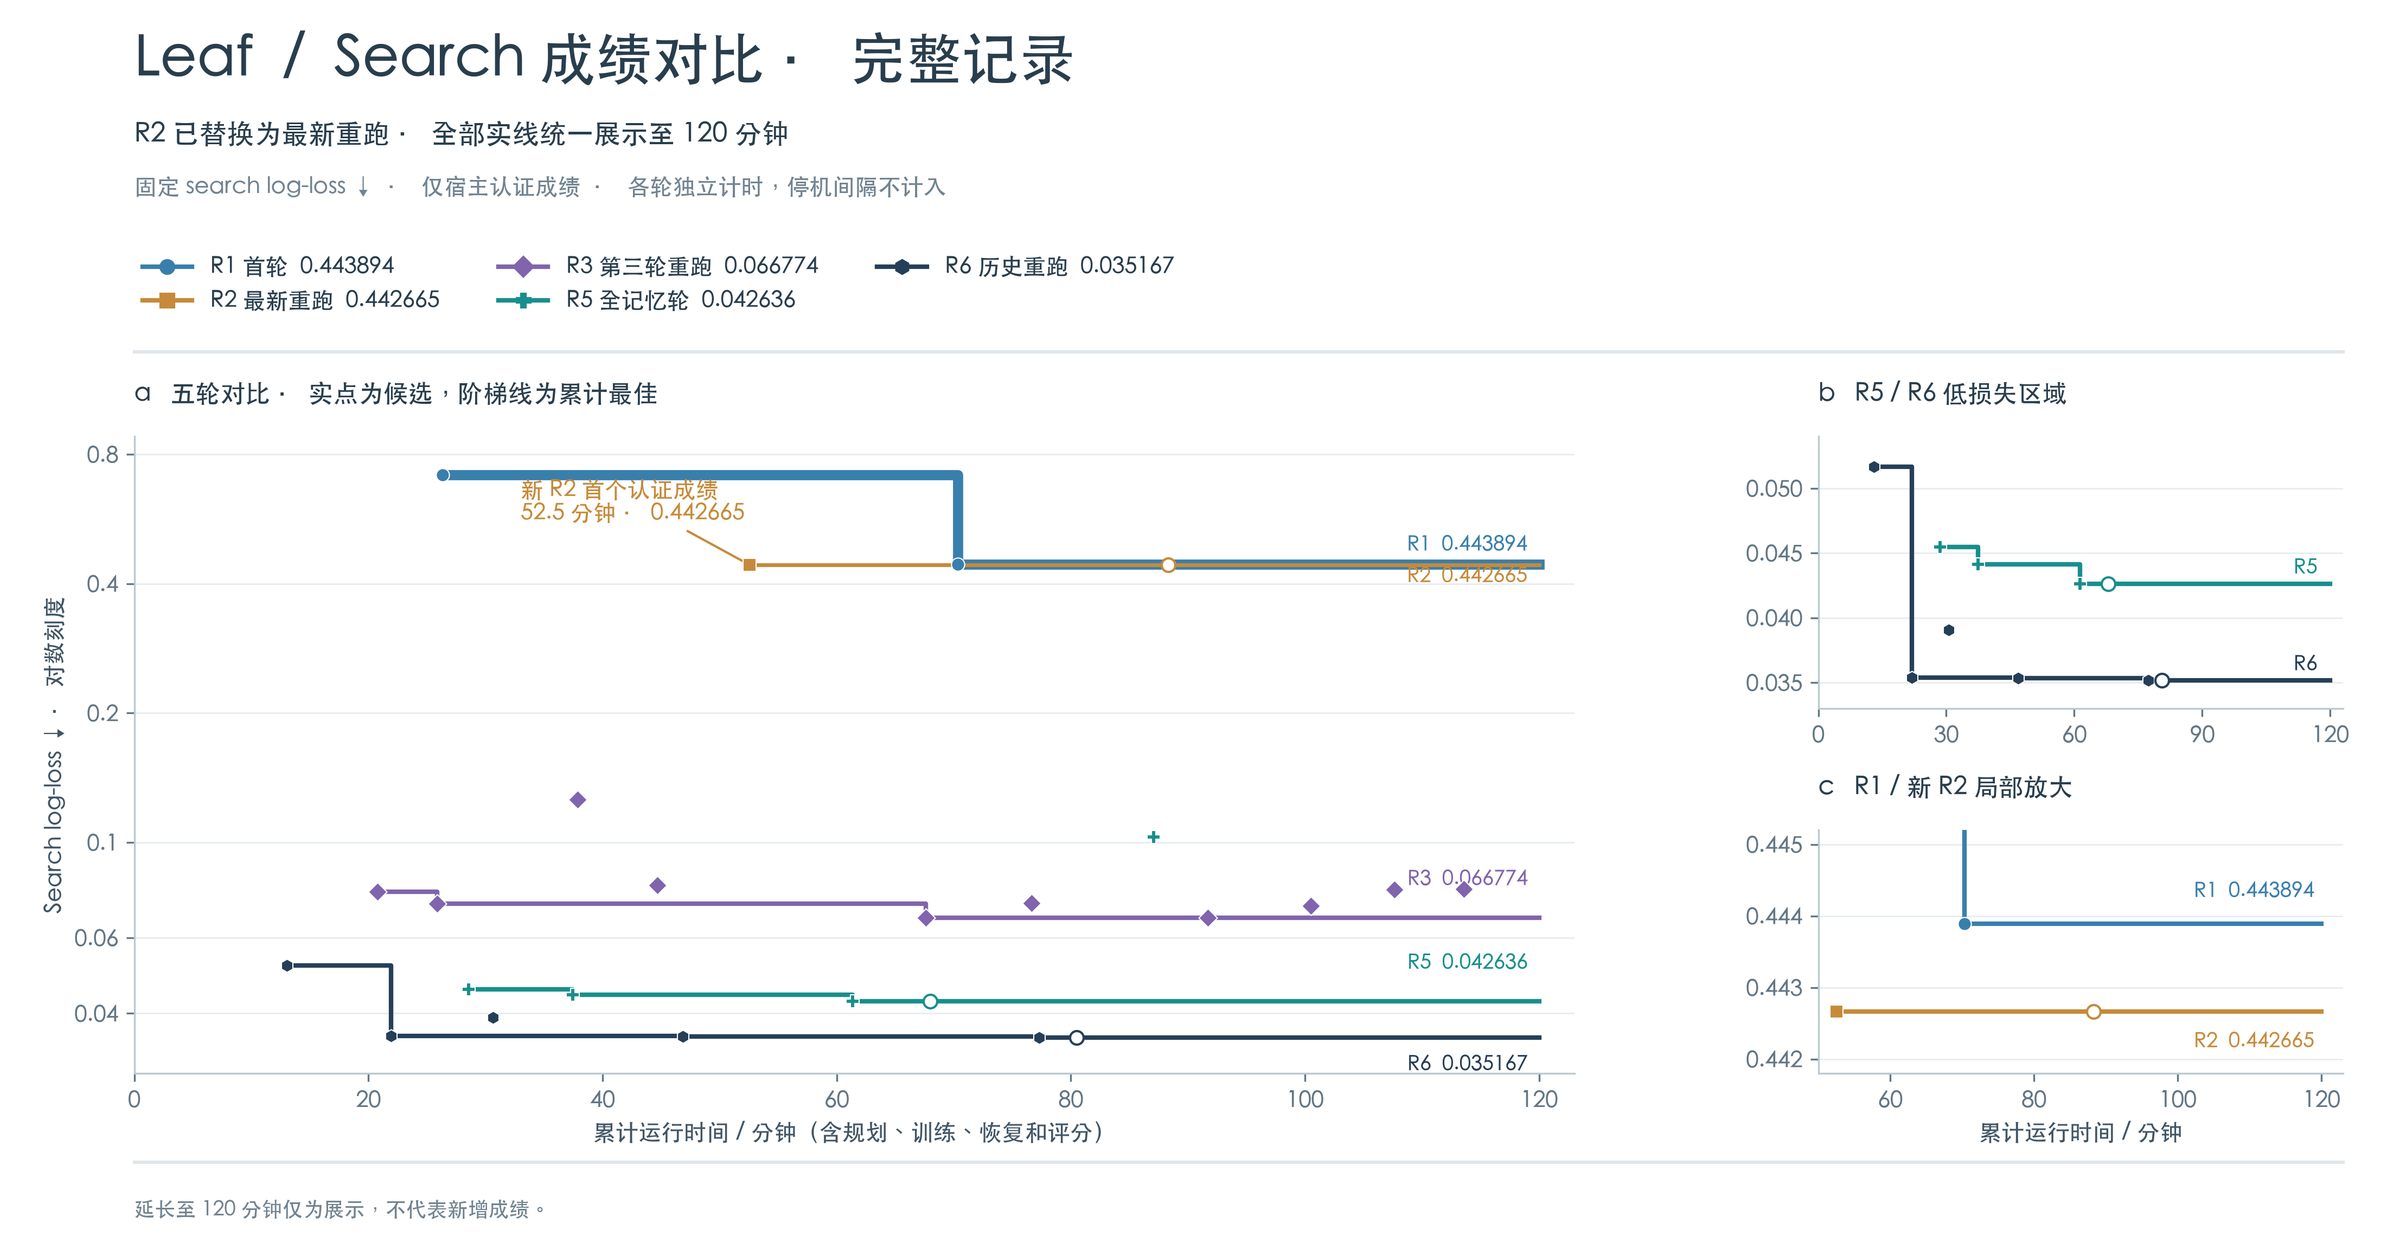
\includegraphics[width=\textwidth]{figures/multiround/mle_leaf_search_rounds.png}
  \caption{MLEvolve, Leaf: Host search log-loss (log scale, lower is better)
  against cumulative runtime for R1 (no memory), R2 (R1 memory, latest rerun),
  R3 (R1+R2), and R5/R6 (91-card cumulative pack; R6 repeats R5's condition).
  Points are certified candidates; step lines are running bests.  Lines are
  extended to 120 minutes for display only.  Panels b and c magnify the
  low-loss region and the R1/R2 overlap.}
  \label{fig:mle-leaf-rounds}
\end{figure*}

\begin{figure*}[t]
  \centering
  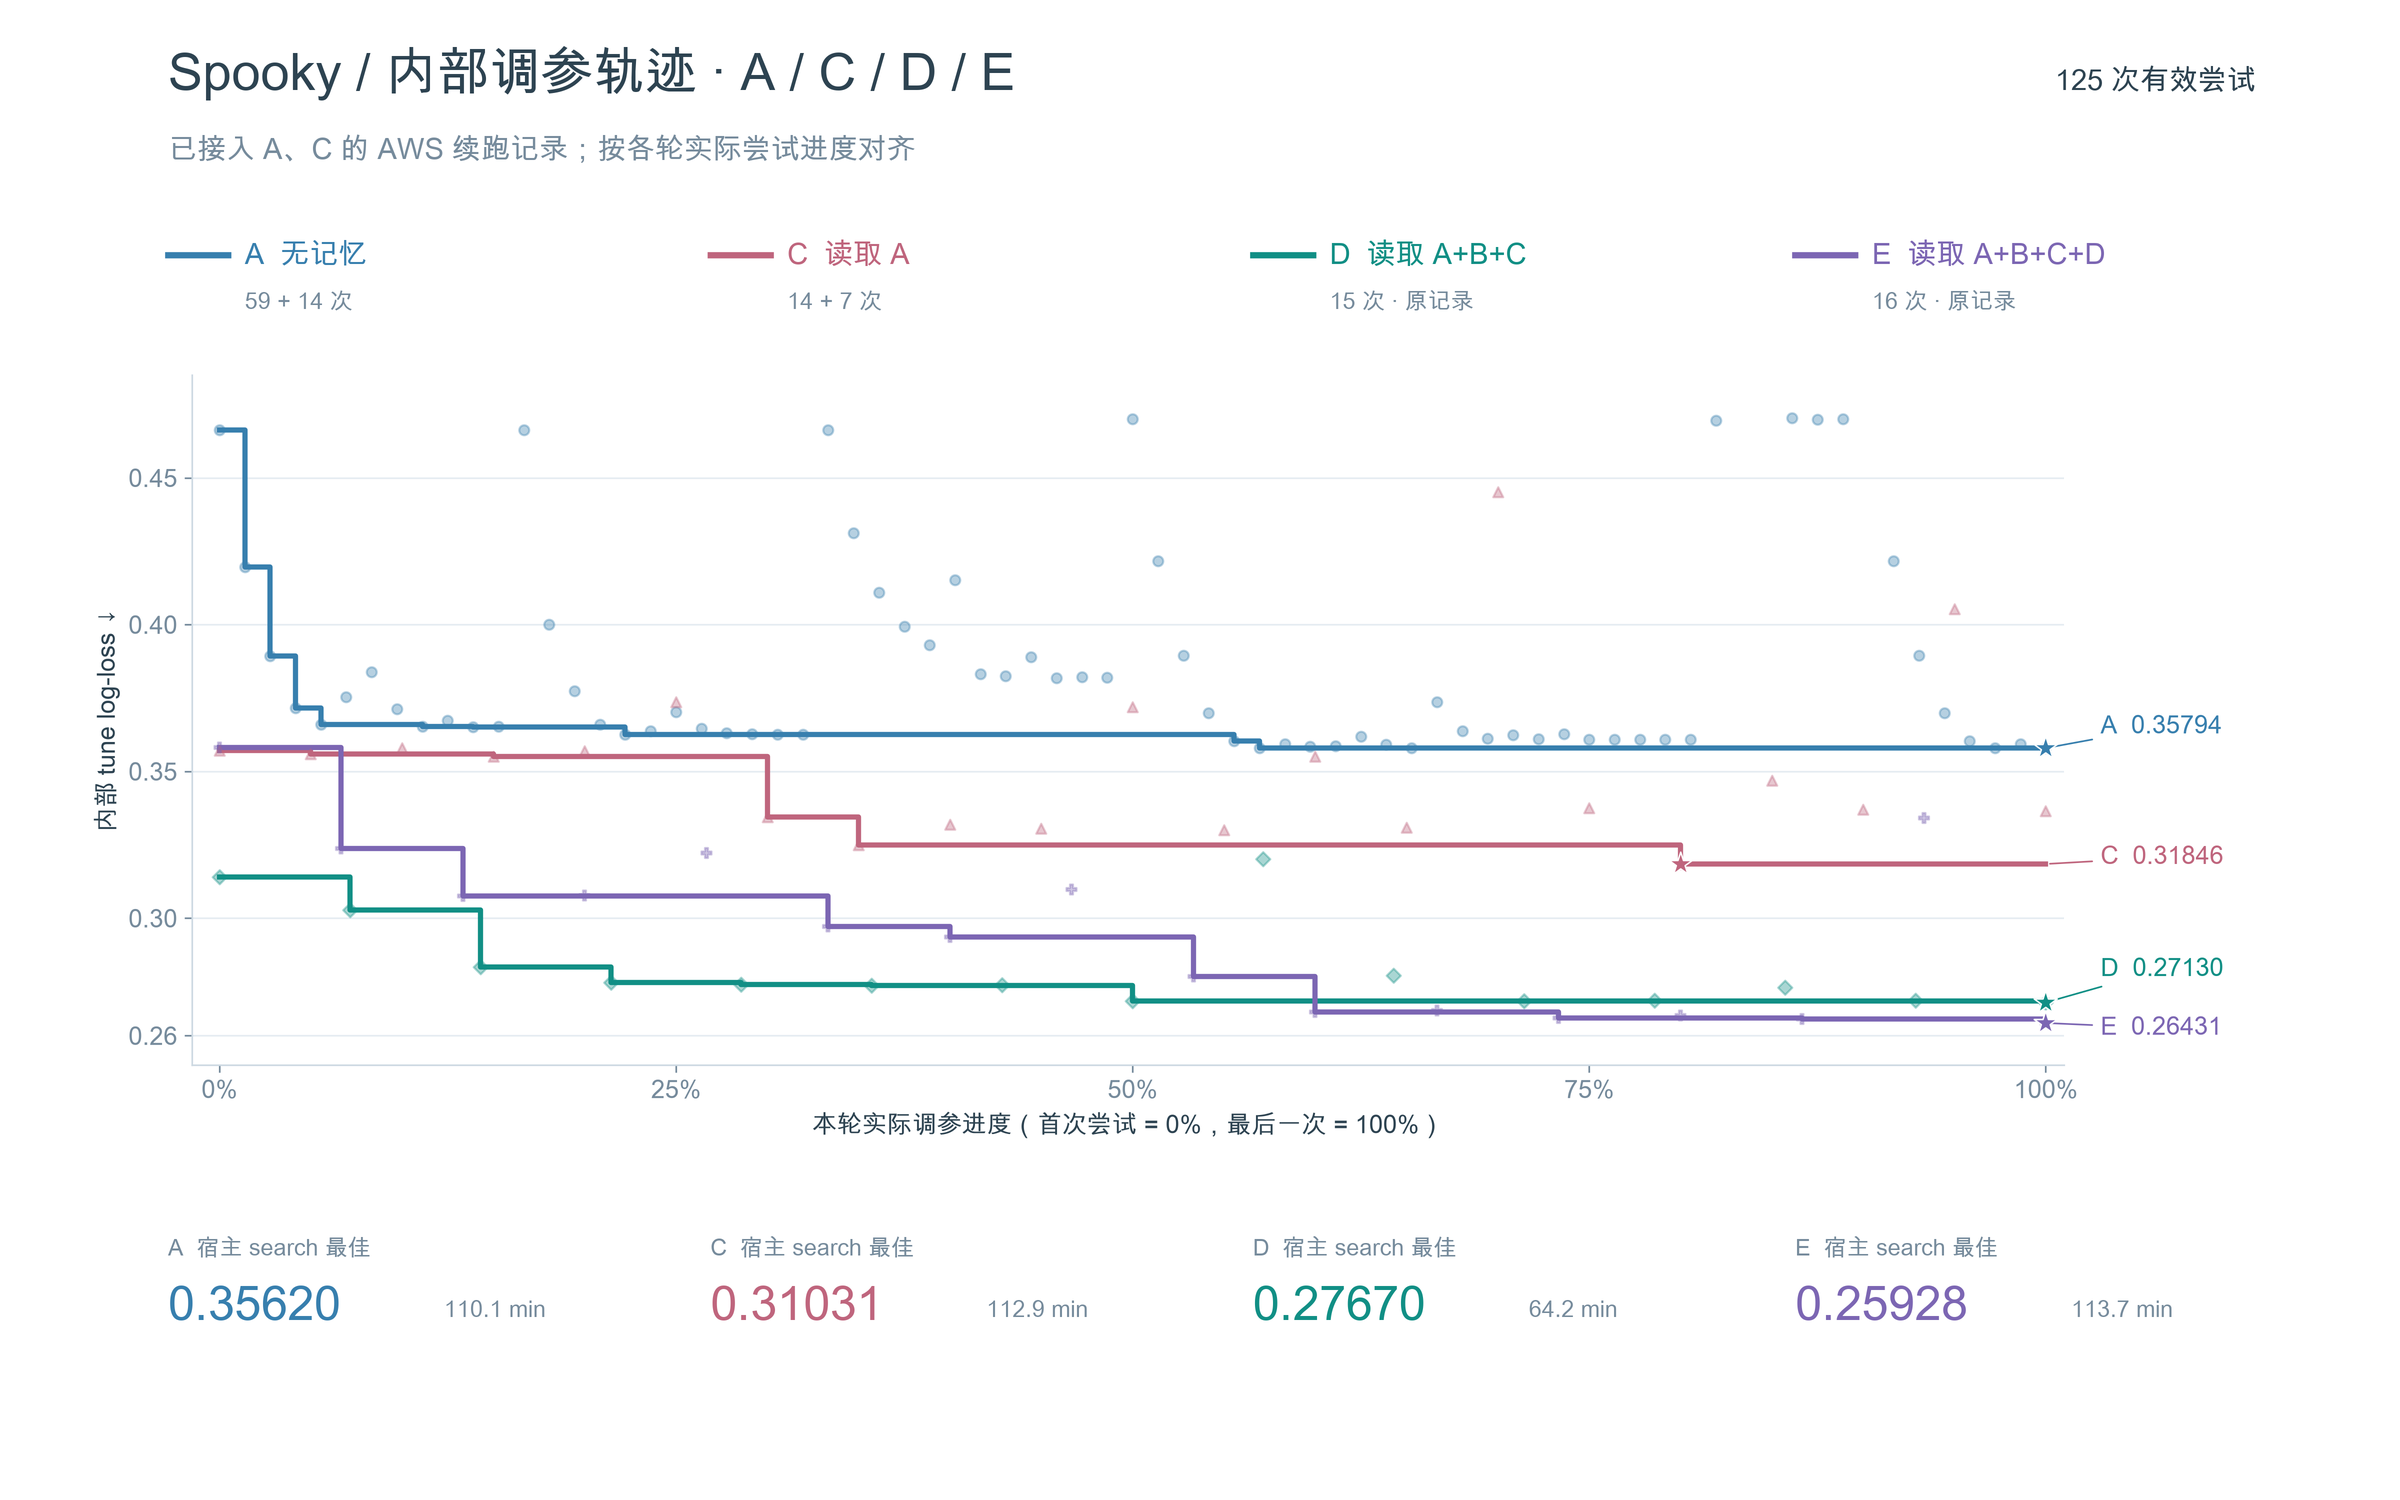
\includegraphics[width=\textwidth]{figures/multiround/mle_spooky_acde_inner.png}
  \caption{MLEvolve, Spooky Author Identification: inner-tuning log-loss
  (lower is better) against normalized attempt progress for A (no memory),
  C (reads A), D (reads A+B+C), and E (reads A+B+C+D); 125 valid trials.
  The footer reports each round's best Host search log-loss and its time.
  Round B is used as a memory source but not plotted.}
  \label{fig:mle-spooky-acde}
\end{figure*}

\begin{figure*}[t]
  \centering
  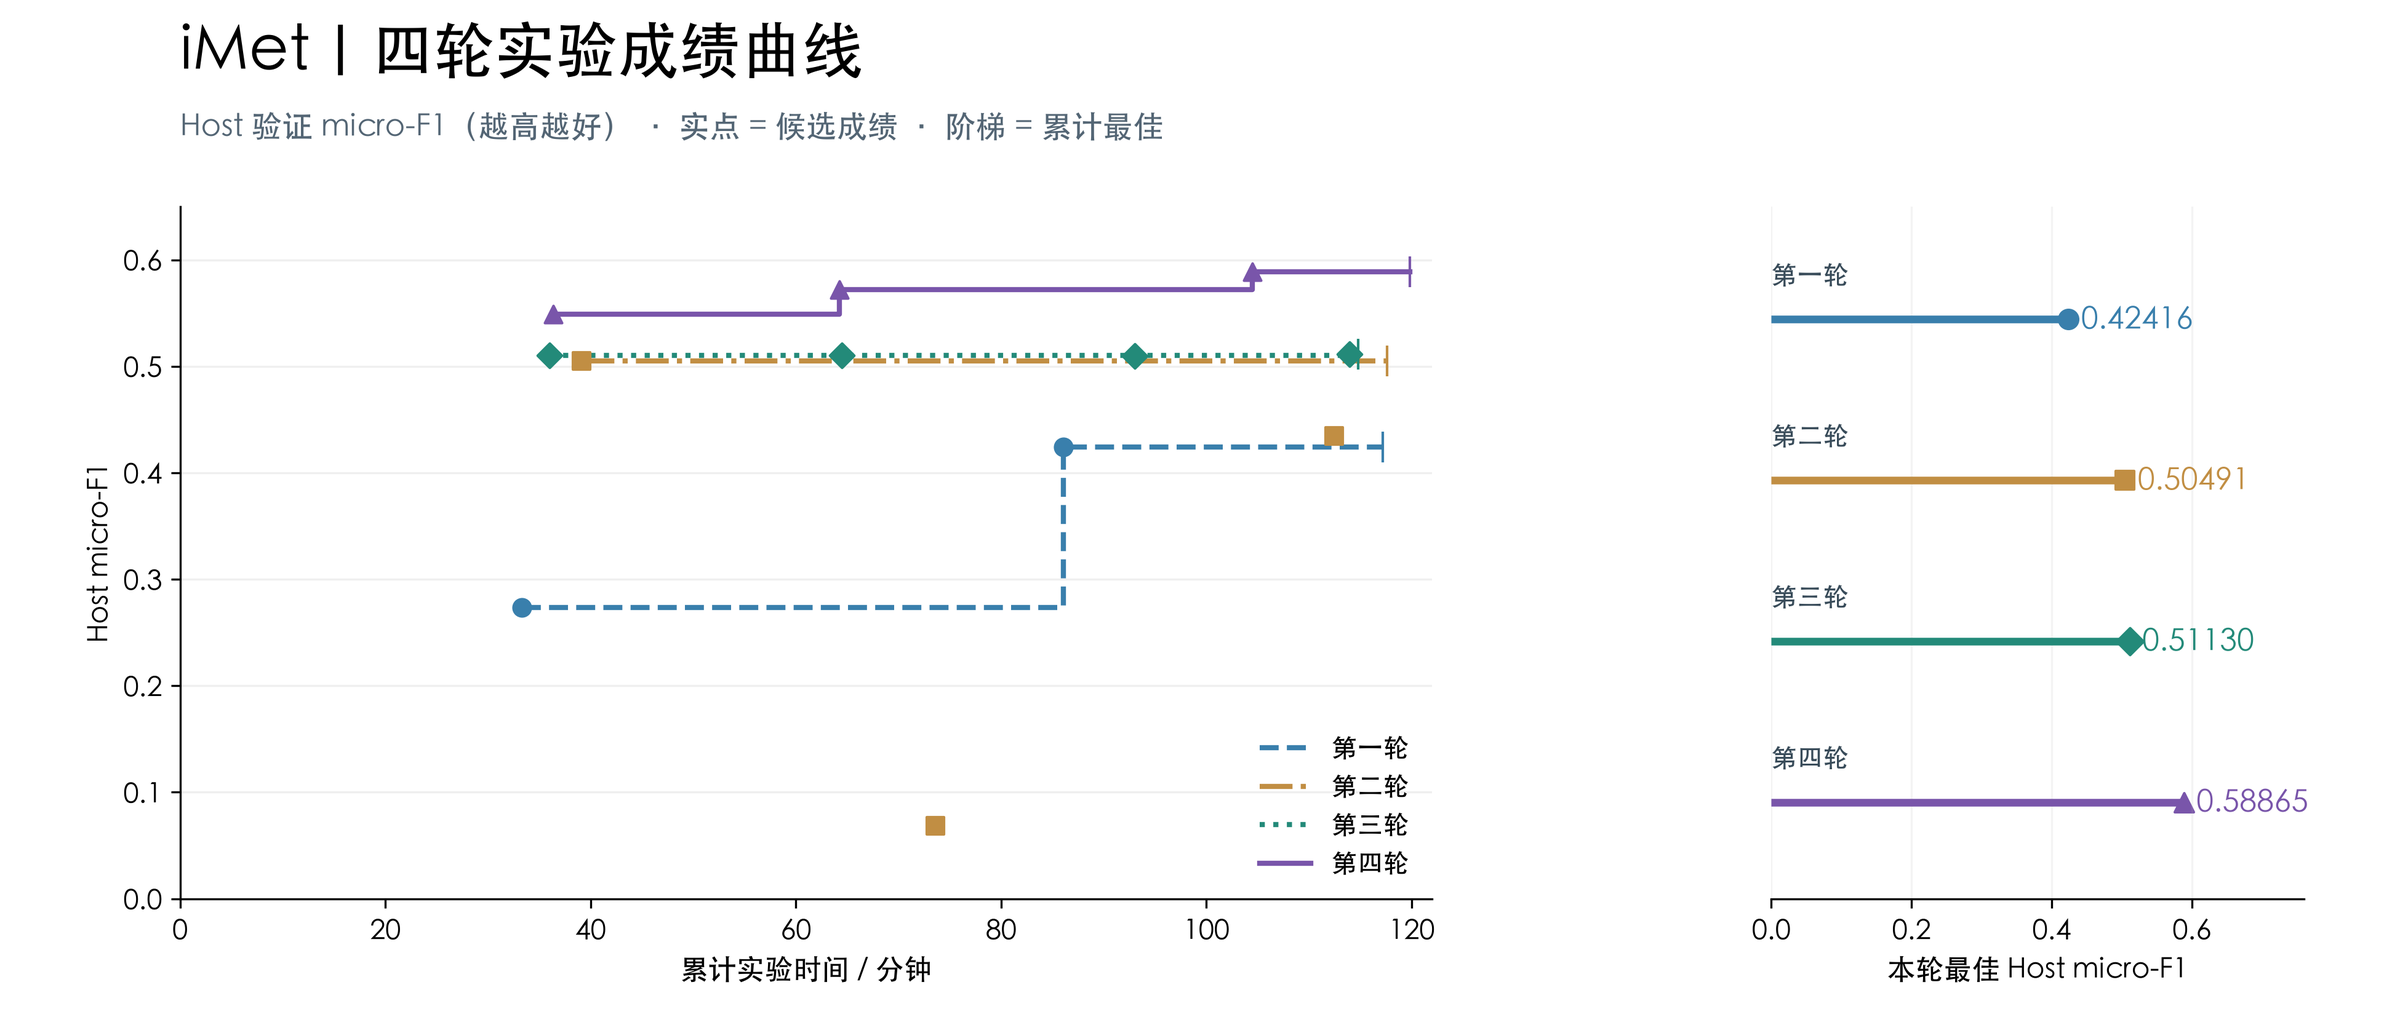
\includegraphics[width=\textwidth]{figures/multiround/mle_imet_four_rounds.png}
  \caption{MLEvolve, iMet 2020 FGVC7 (3{,}474 attributes): Host micro-F1
  (higher is better) against cumulative runtime for four rounds with
  increasing memory (none; R1; R1+R2; R1+R2+R3).  Points are
  checkpoint-validated, Host-recomputed candidates; step lines are running
  bests; the right panel shows each round's best.}
  \label{fig:mle-imet-rounds}
\end{figure*}

\begin{figure*}[t]
  \centering
  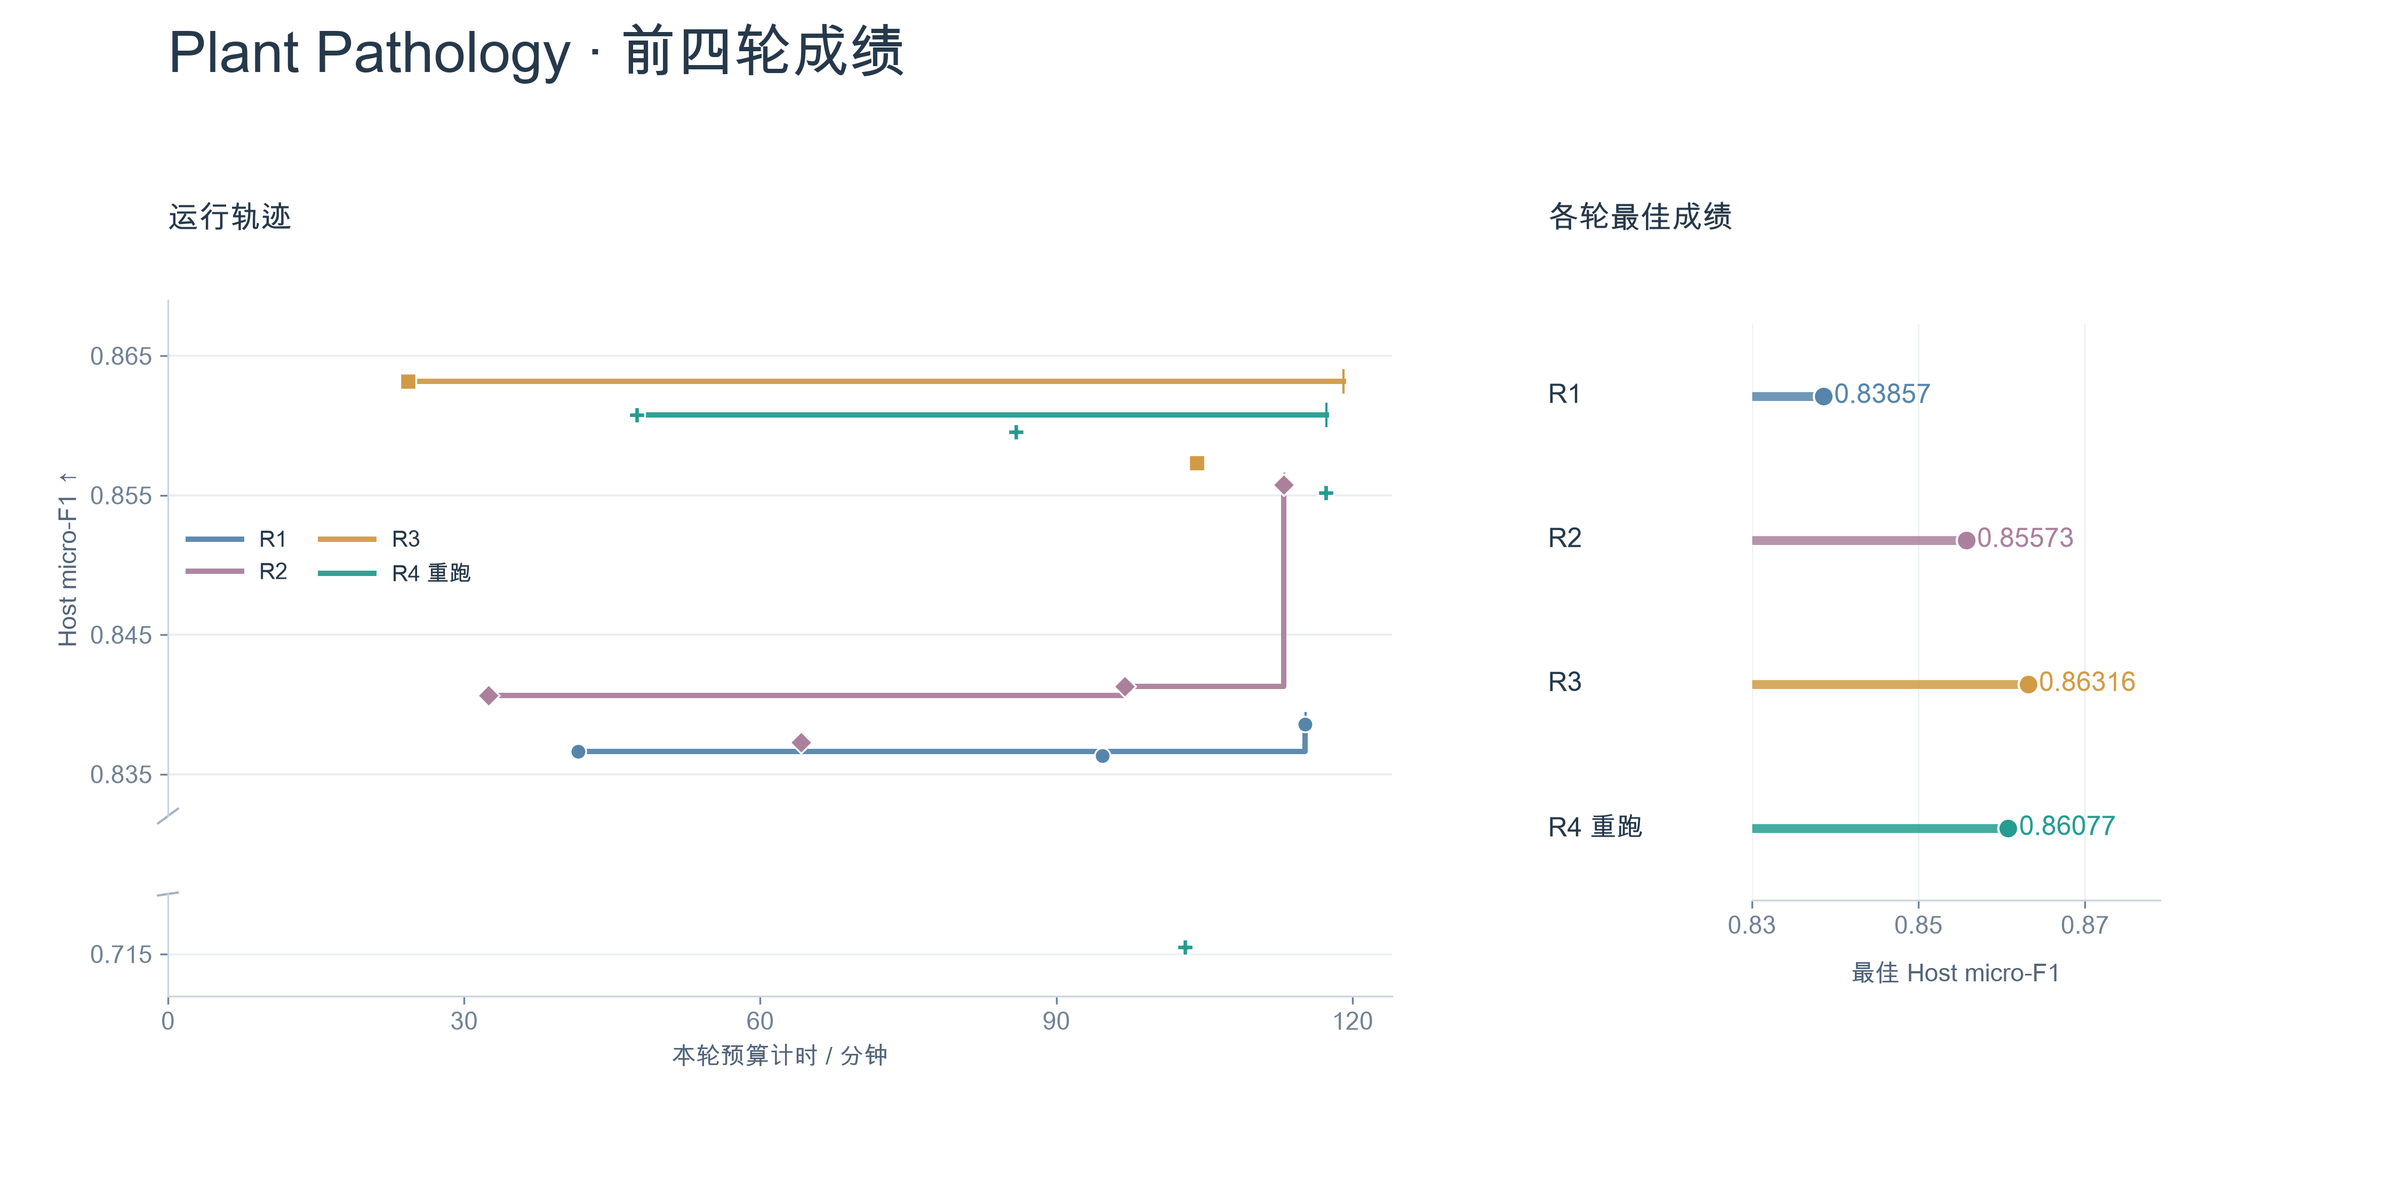
\includegraphics[width=\textwidth]{figures/multiround/mle_pp21_four_rounds.png}
  \caption{MLEvolve, Plant Pathology 2021 FGVC8 (six labels): Host micro-F1
  (higher is better) against budgeted runtime for R1 (no memory), R2 (R1),
  R3 (R1+R2), and the R4 repeat (R1+R2+R3).  The broken axis keeps one
  low-scoring R4 candidate (0.716) visible.}
  \label{fig:mle-pp21-rounds}
\end{figure*}

\begin{figure*}[t]
  \centering
  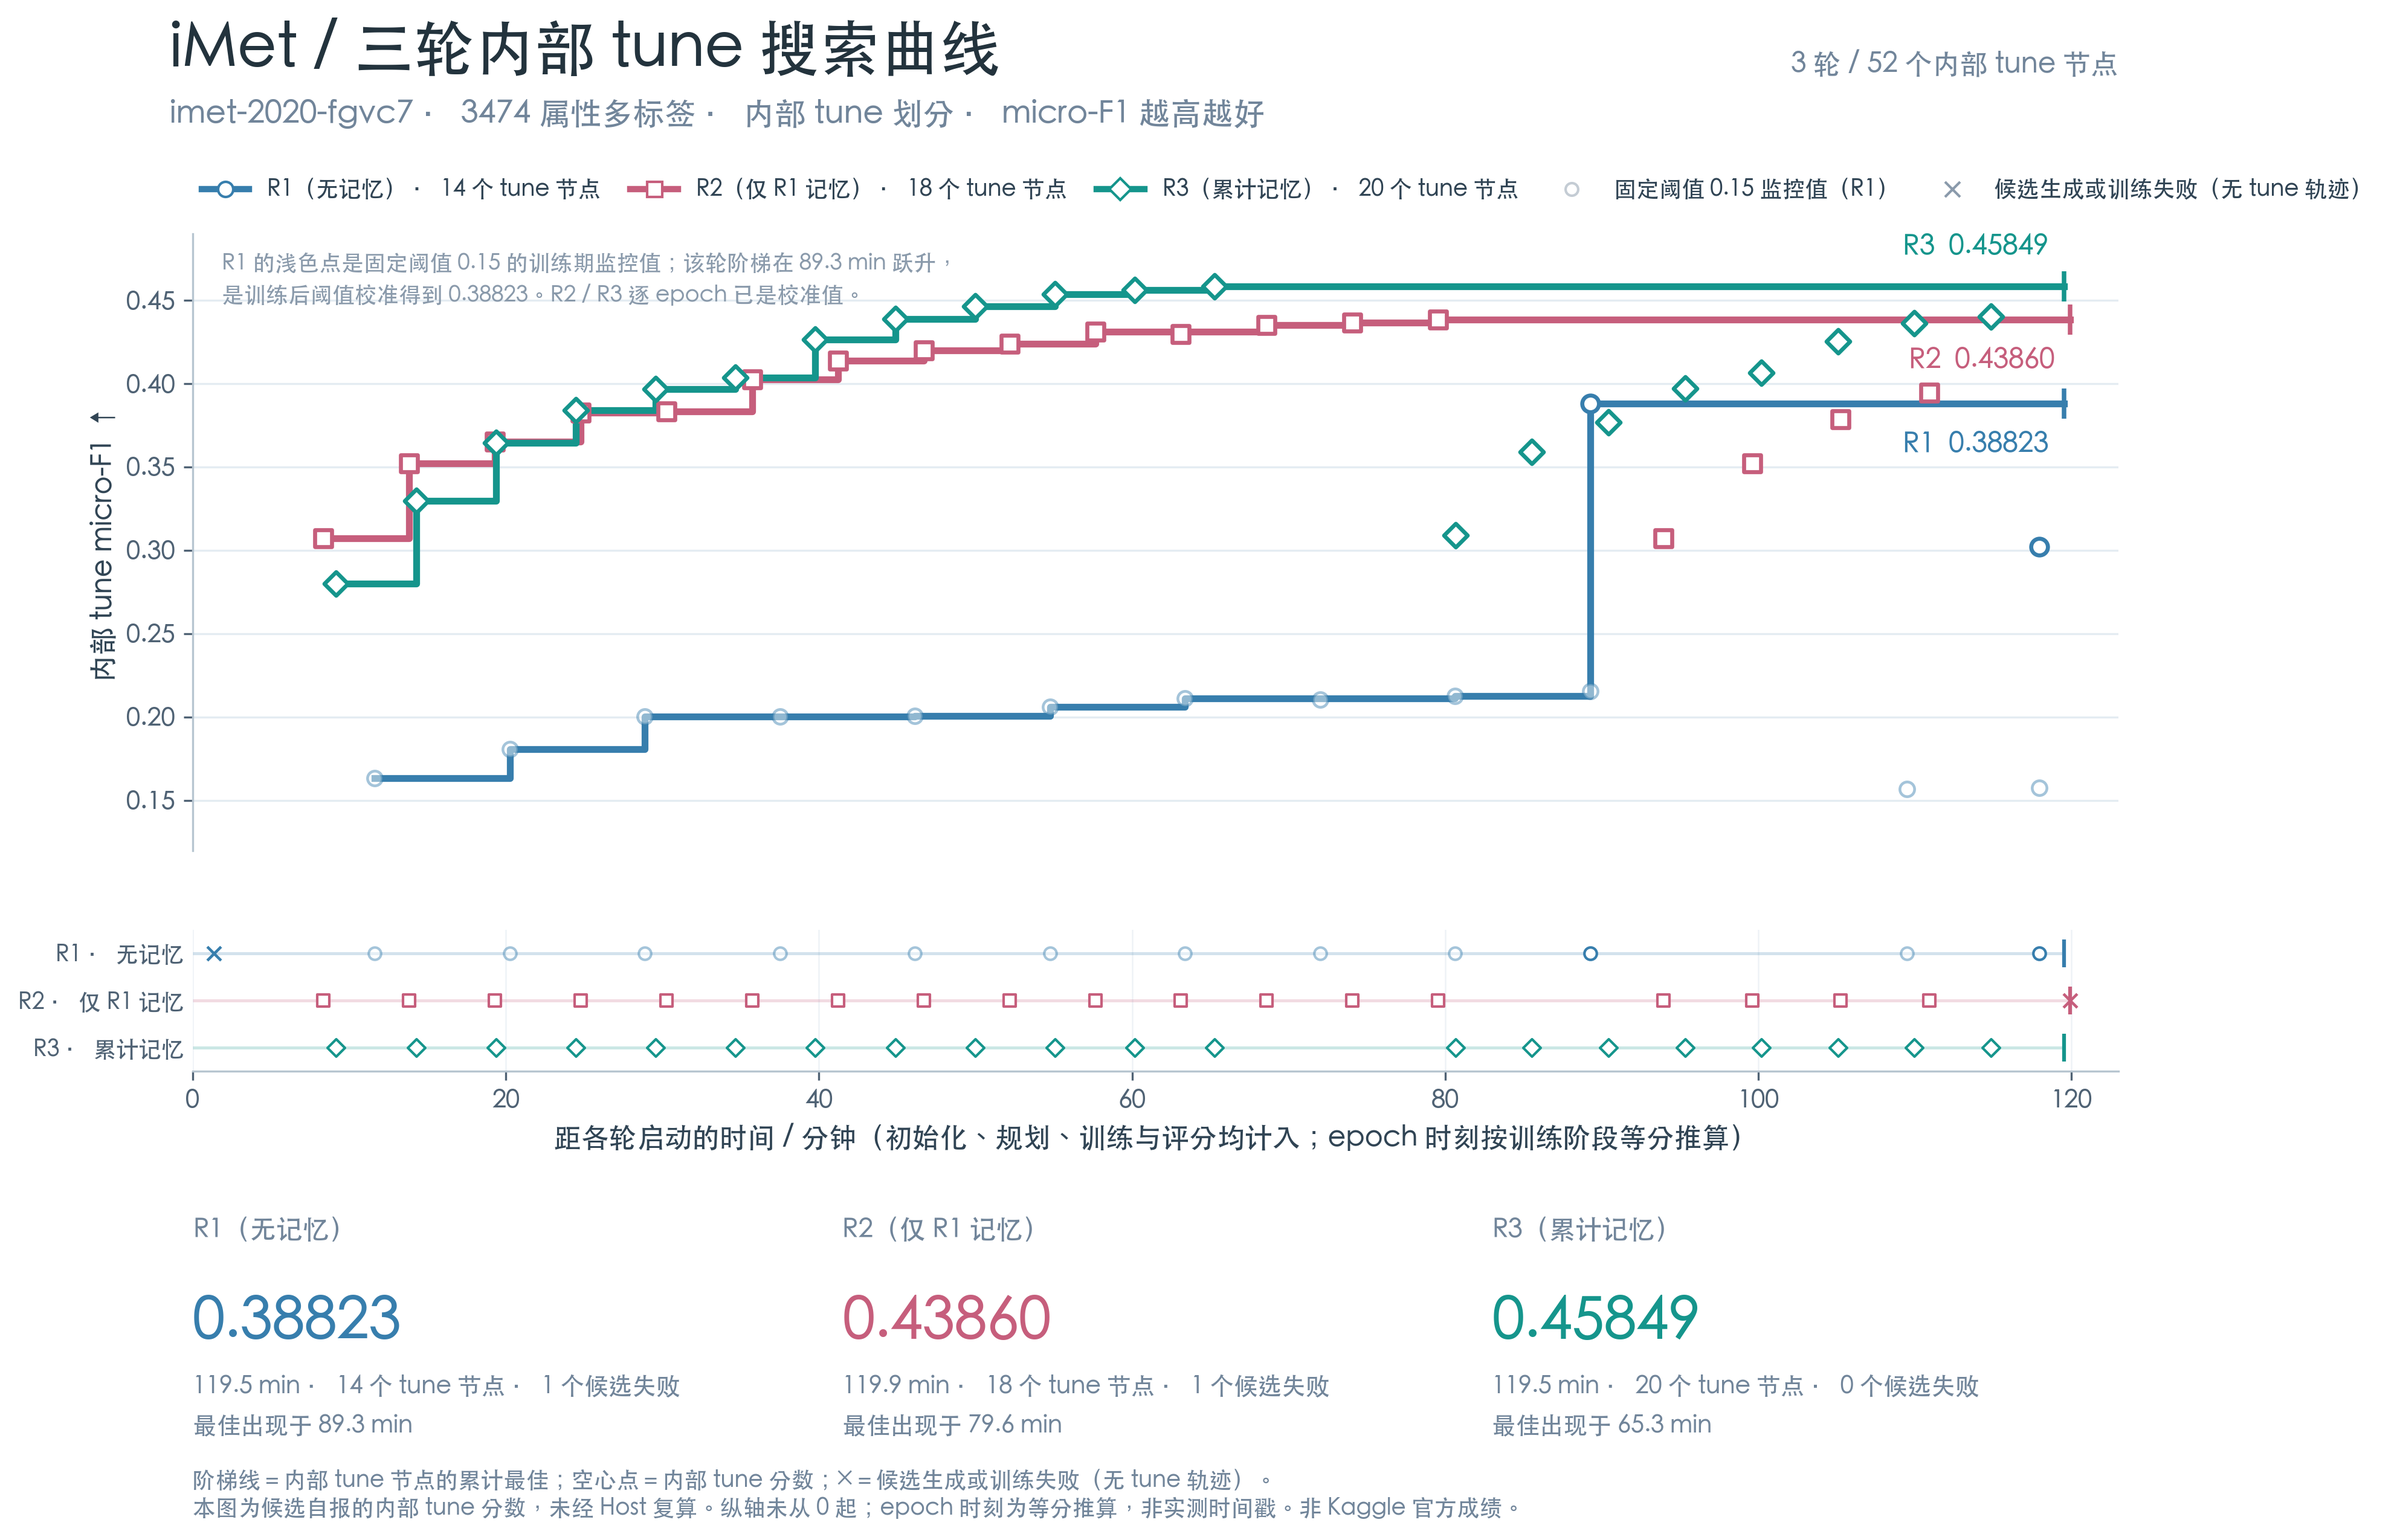
\includegraphics[width=\textwidth]{figures/multiround/ar_imet_three_rounds_tune.png}
  \caption{autoresearch, iMet 2020: internal tune micro-F1 (higher is better)
  for R1 (no memory), R2 (R1 memory only), and R3 (cumulative R1+R2), with
  52 tune nodes in total.  R1's light points are a fixed-threshold (0.15)
  training monitor and are not comparable with the calibrated values; epoch
  times are interpolated within each training stage.  The y-axis does not
  start at zero.}
  \label{fig:ar-imet-rounds}
\end{figure*}

\begin{figure*}[t]
  \centering
  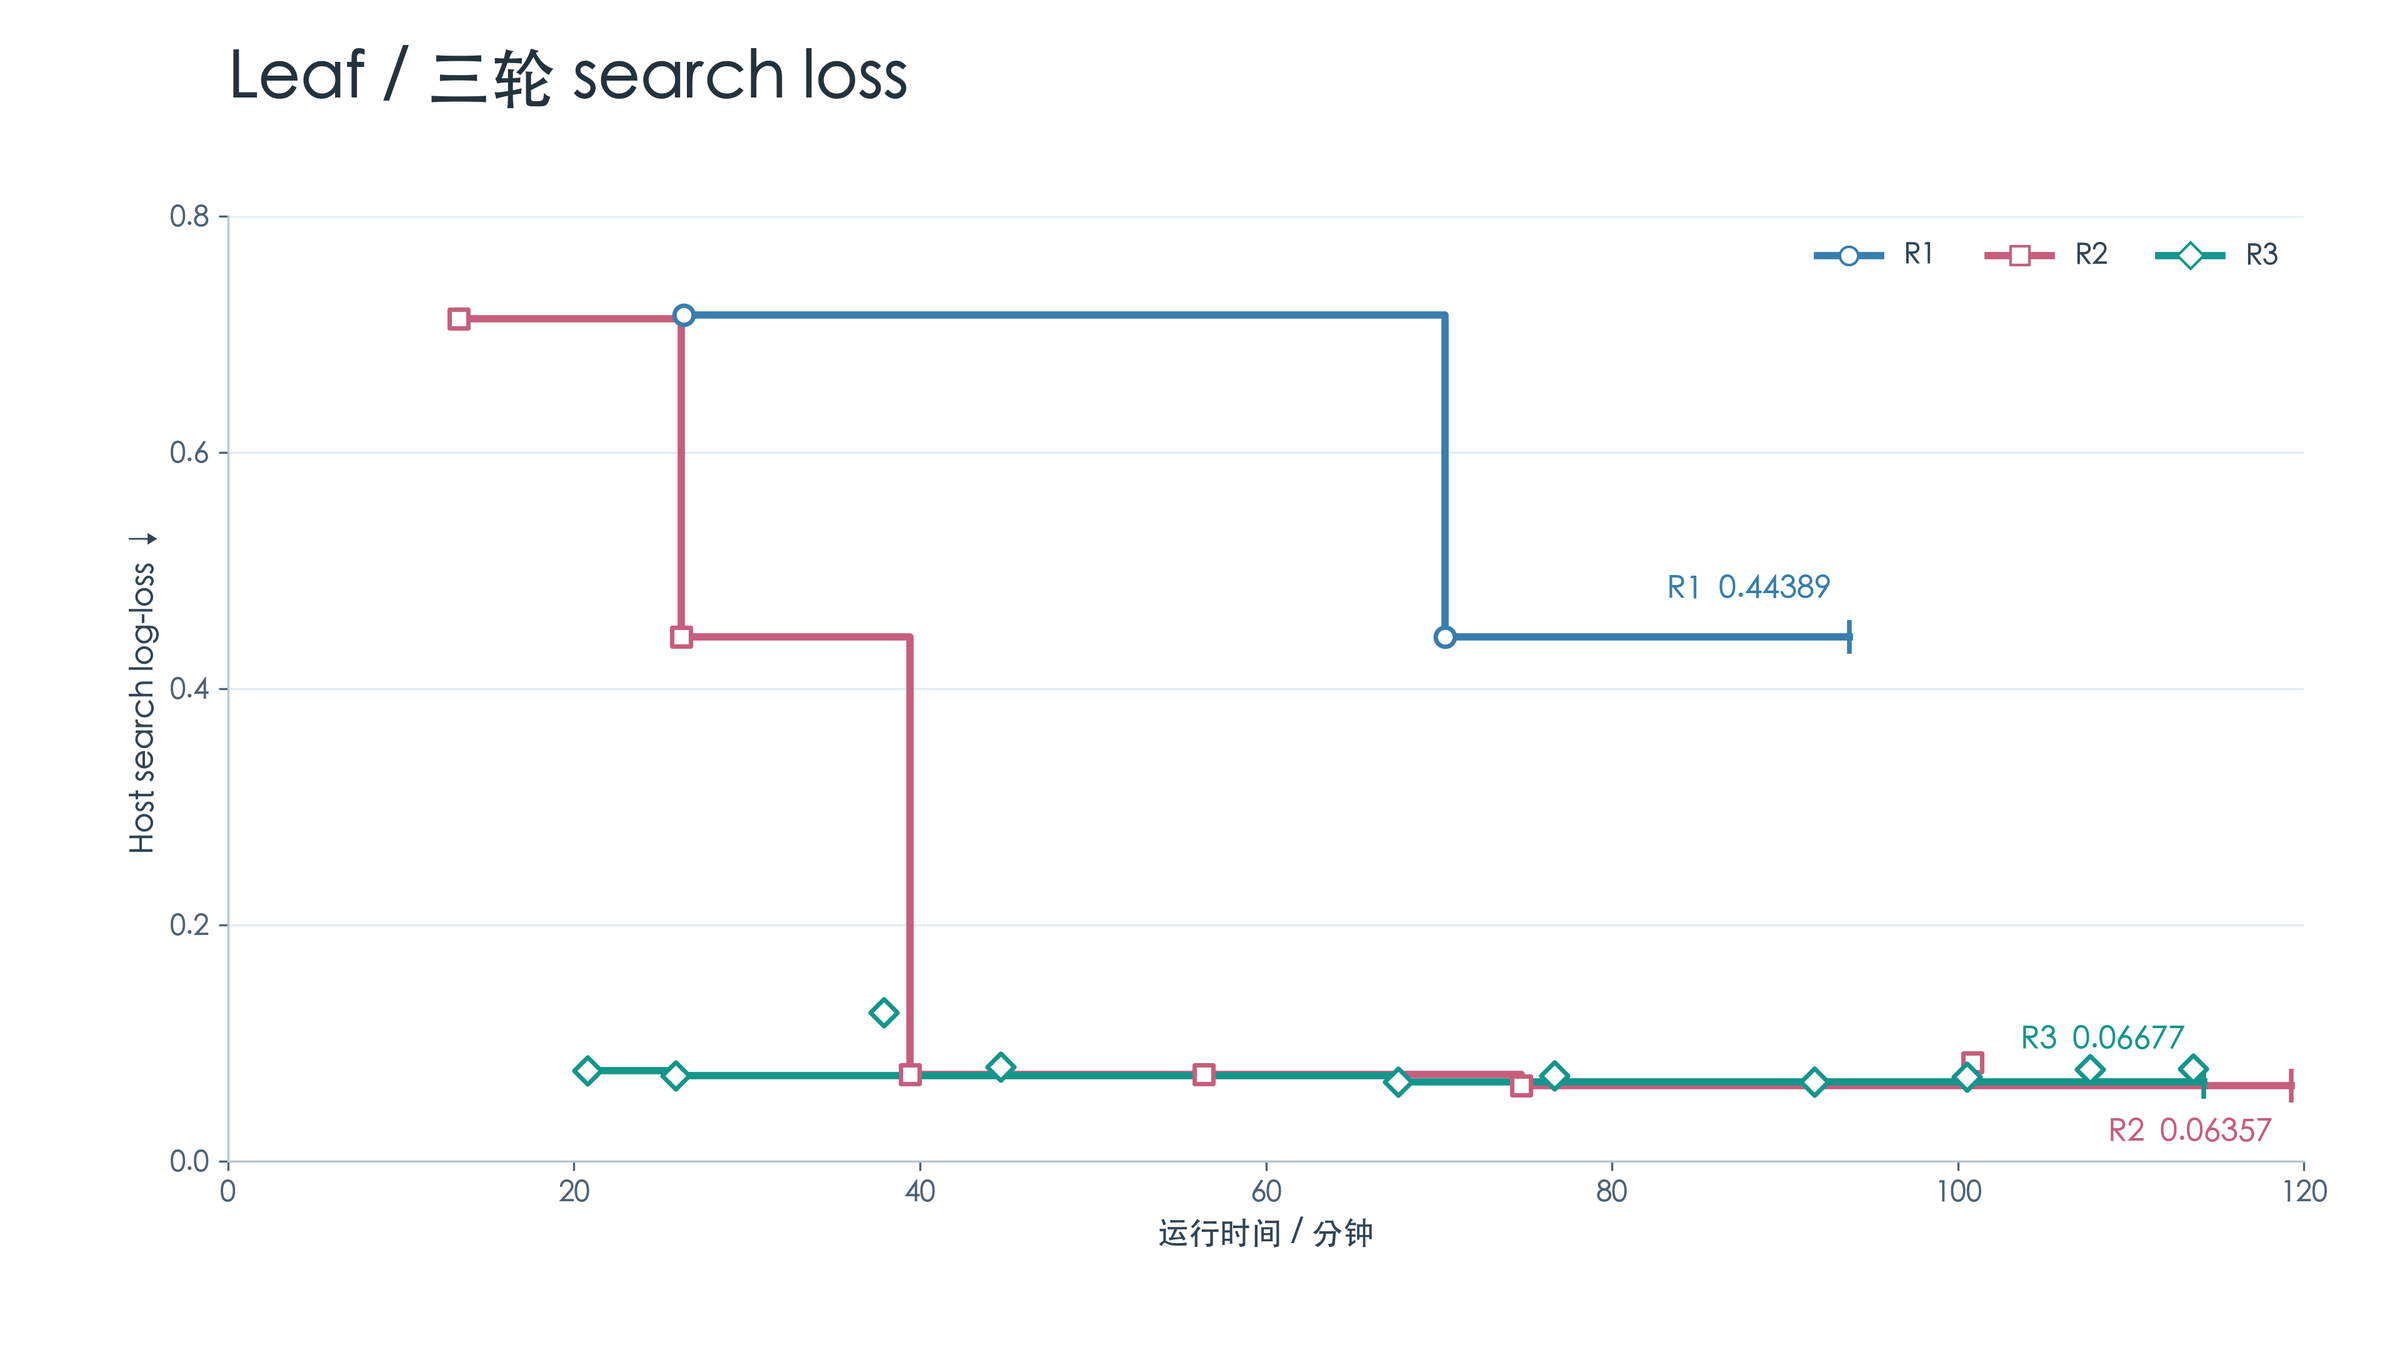
\includegraphics[width=0.85\textwidth]{figures/multiround/ar_leaf_three_rounds.png}
  \caption{Leaf, mixed series: Host search log-loss against runtime.  R2 is an
  autoresearch round that reads memory distilled from the MLEvolve R1; R1 and
  R3 are the MLEvolve rounds of Figure~\ref{fig:mle-leaf-rounds} (R3 reads the
  original MLEvolve R2, not the plotted autoresearch R2).}
  \label{fig:ar-leaf-rounds}
\end{figure*}

\begin{figure*}[t]
  \centering
  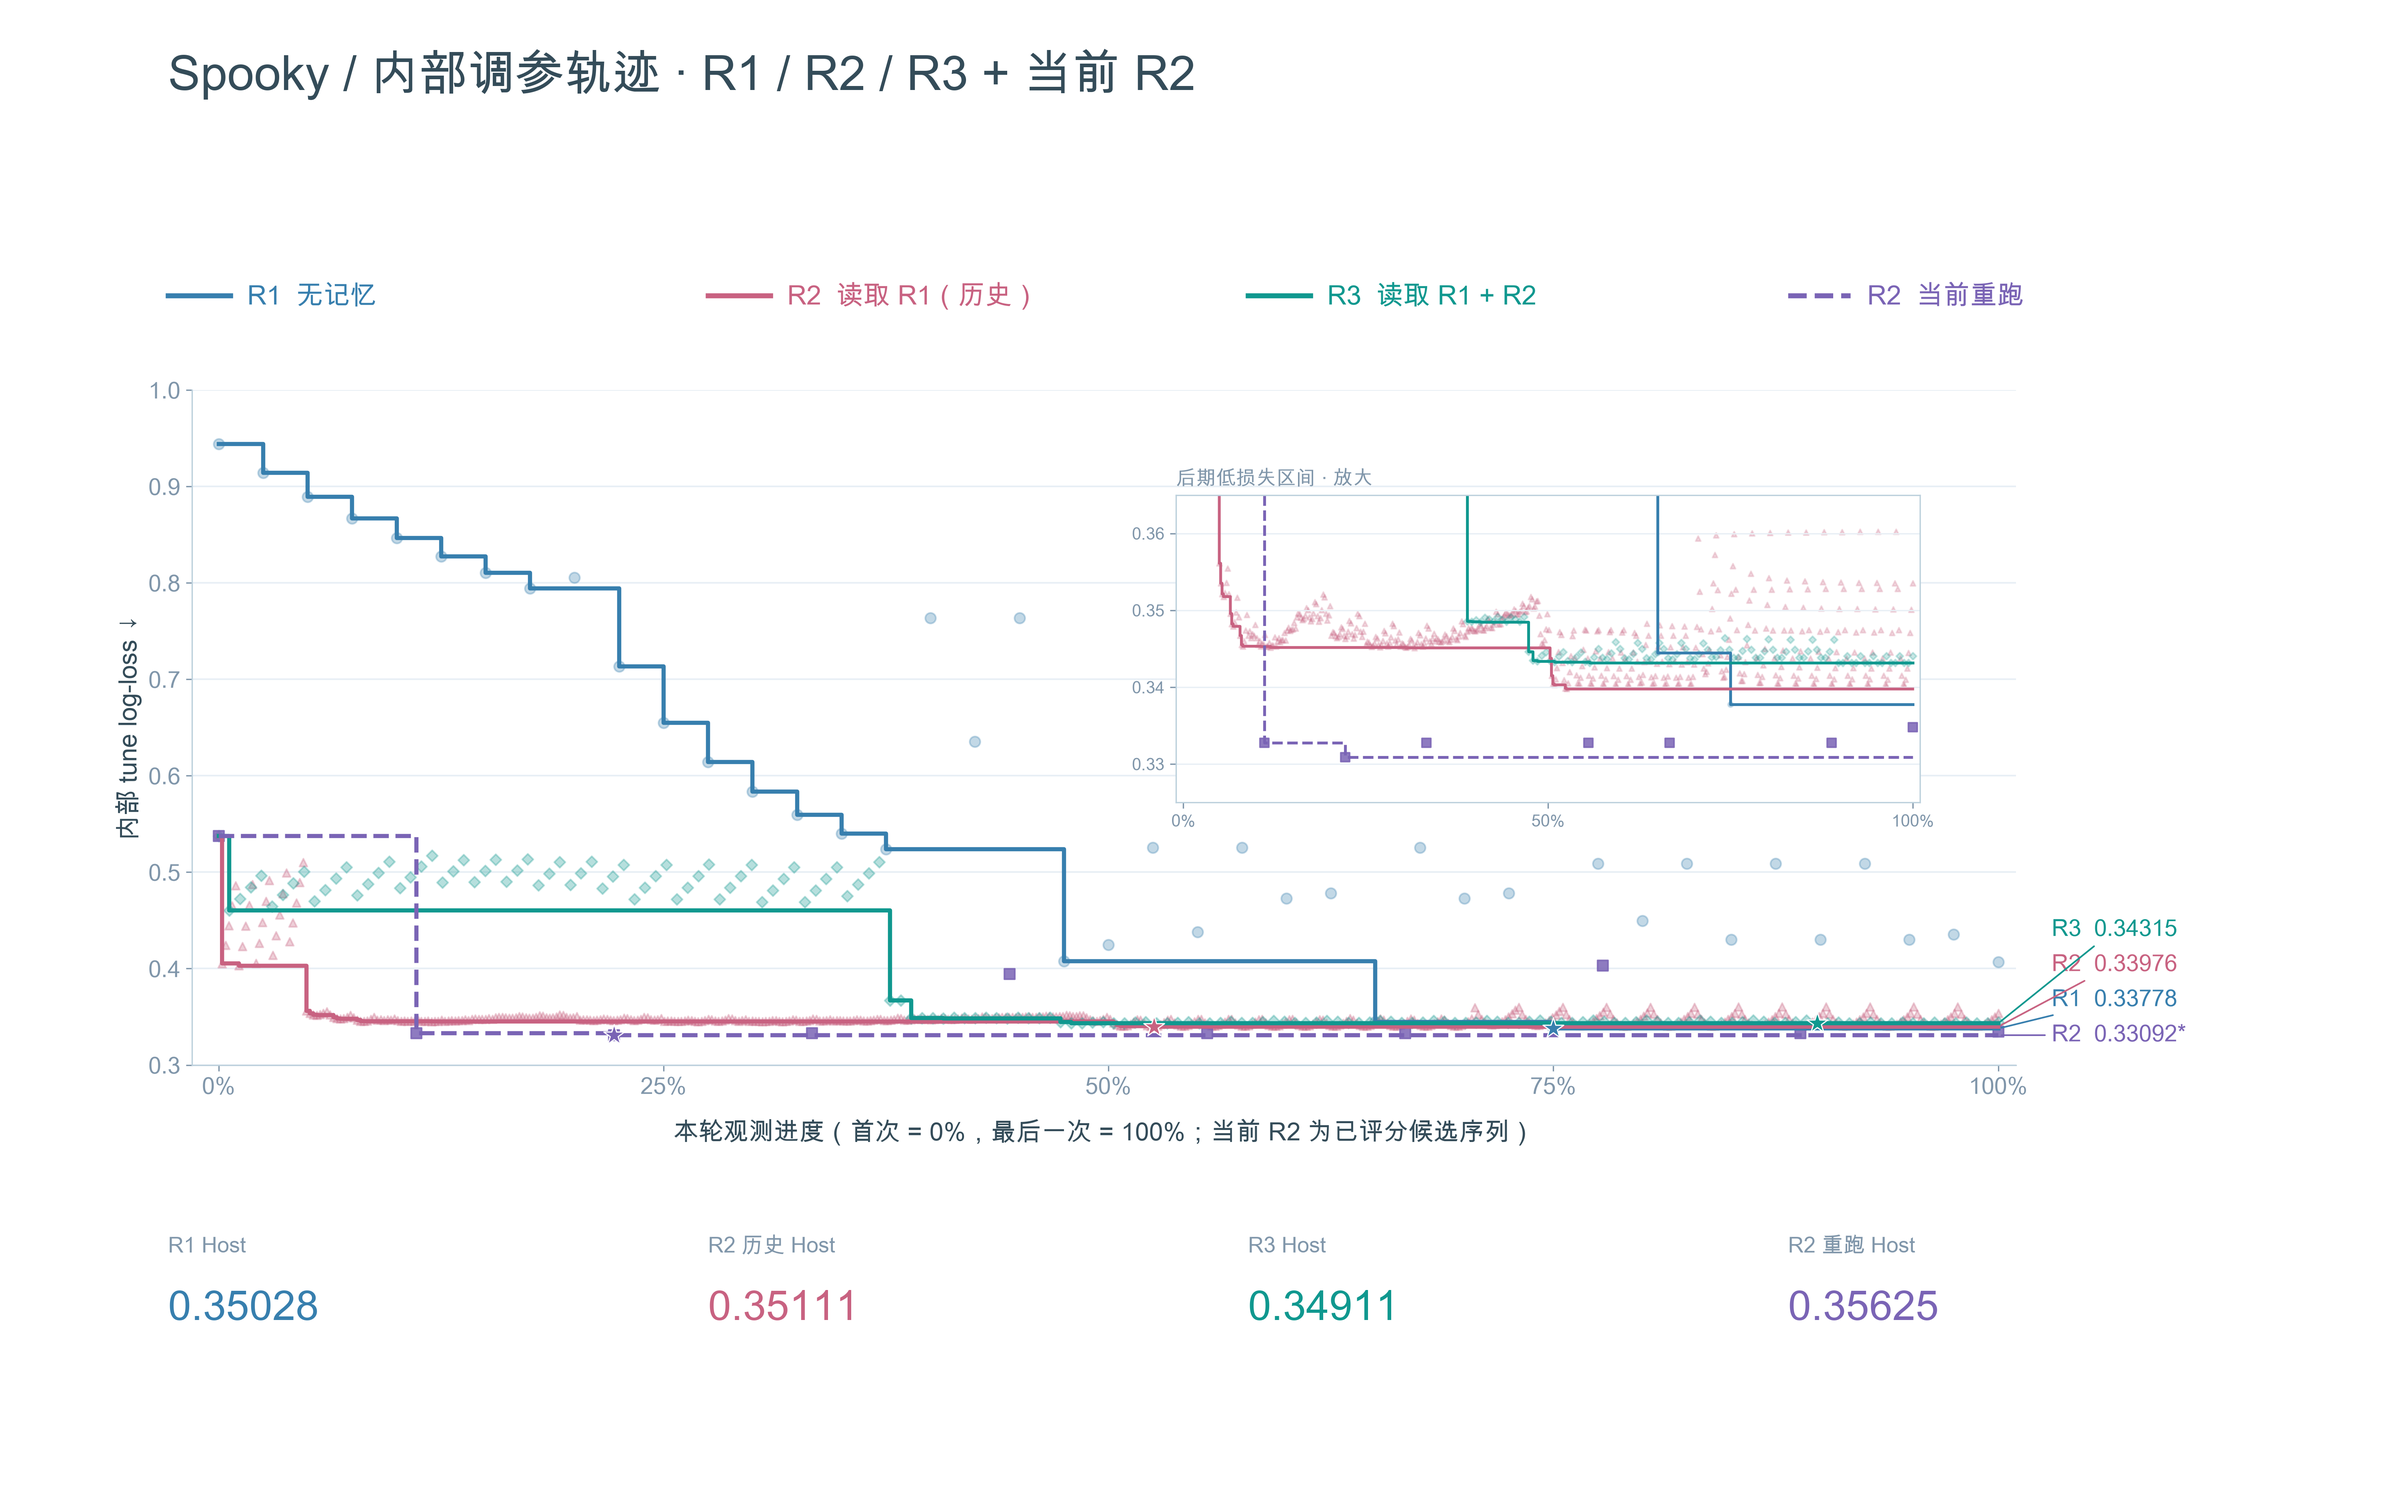
\includegraphics[width=\textwidth]{figures/multiround/ar_spooky_rounds.png}
  \caption{Spooky, mixed series: inner tune log-loss against normalized
  observation progress.  R1 is a historical MLEvolve run truncated to the
  7{,}200\,s budget; R2 (reads R1) and R3 (reads R1+R2) are autoresearch
  rounds; the dashed ``current R2'' is an autoresearch rerun that reads a new
  autoresearch no-memory R1 and stopped at about 60 minutes on a provider
  error.  The footer reports Host search log-loss.}
  \label{fig:ar-spooky-rounds}
\end{figure*}
\FloatBarrier


\subsection{Structural geometry is useful but not a downstream result}

On the clean run-tree diagnostic, Poincar\'e coordinates outperform their
Flat-Twin for parent lookup (MRR 0.3775 vs. 0.2813) and transition-to-SOP
signposts (0.5716 vs. 0.5435), while Flat-Twin is better for pure-distance debug
child recovery (0.4738 vs. 0.3870).  Explicit parent--child graph expansion
recovers debug children and local-best lineage with score 1.0 by construction.
The correct operational conclusion is that upward lineage and explicit graph
navigation have different primitives.  These diagnostics do not override the
causal Debug result: that benchmark intentionally uses the Flat-Twin carrier and
does not compare hyperbolic with Euclidean geometry.

\FloatBarrier
\section{Failure Analysis}
\label{sec:failure}

\subsection{Historical three-model replay}

The most informative case is a historical Spooky ensemble combining
DeBERTa-v3-large, XGBoost, and Logistic Regression with word/character TF--IDF
and punctuation/stylometric features.  The reported value 0.2013 was attractive,
and exact replay successfully found the source.  However, audit identified two
independent defects:

\begin{enumerate}[leftmargin=*,itemsep=1pt]
  \item a punctuation vectorizer was fit on a union containing validation/test
  rows, creating transductive preprocessing leakage; and
  \item ensemble weights were searched on the same validation labels used for
  the reported score, creating selection bias.
\end{enumerate}

The source is therefore a \texttt{blocked\_exact\_source\_repair\_seed} with no
GPU execution, metric, or rank eligibility.  The value 0.0494 seen in an earlier
trace was a parsing/diagnostic artifact rather than a valid score and is also
excluded.

\subsection{Why free-form repair repeatedly failed}

Early repair attempts treated a five-part protocol rewrite as two ordinary
debug generations.  One attempt introduced a nested split but sliced feature
arrays by length rather than propagating real sample indices.  Another restored
executability by returning to validation-set weight selection.  Later staged
versions exposed additional engineering failures: stage indices consumed a
global two-attempt budget; empty LLM programs left in-flight reservations
unreleased; generated code invented provenance APIs; apparent OOF code lacked
fit-scope and exactly-once coverage evidence; and selection code sometimes
failed to use the recorded global OOF metric.

These failures motivated the current design rather than serving as successful
results.  They also show why increasing an unconstrained retry count is not a
principled fix.  The repair agent must receive stage-specific rejection feedback,
use a finite API, preserve the method, and release reservations atomically after
failure.

\subsection{What the completed online study can and cannot establish}

The formal study establishes assigned-condition traceability, host-owned
evaluation, Result Fact retention, and a negative superiority decision under a
frozen gate.  It does not establish that injected historical experience caused
the four favorable available-pair deltas.  Static and runtime actuation are
required for an Adoption Edge, and a memory-on/off counterfactual is additionally
required for a Causal Edge; the randomized Full-versus-No-Memory system contrast
does not substitute for those receipts.  Earlier self-reported values such as
0.319 or 0.363 remain search telemetry, not formal terminal scores.

The r11 partial shadow artifact remains excluded even though a later corrected
shadow/canary completed.  Likewise, post-result semantic-overlap, crash-safety,
empty-pack, tamper, and reporting fixes are supported only as engineering
regressions.  They neither rewrite the 45 formal outcomes nor receive credit in
the effect estimate.

\section{Limitations and Falsification Plan}

\paragraph{Evaluation scale and missingness.}
The stage track contains 120 episodes, but the causal Debug set contains only 38
episodes from 12 source runs and remains retrospective.  The formal online study
adds only three target tasks and three seeds per task.  Of nine Full--No-Memory
assignments, just four are score-estimable and Taxi has none.  This is
insufficient for a broad MLE claim or a stable task-level uncertainty estimate.

\paragraph{Silver failure labels and development visibility.}
Failure signatures are generated by a deterministic benchmark-side code path,
but its categories are semantically aligned with the production matcher.  The
memory graph was also visible during system development.  A paper-grade
generalization claim requires a frozen router, unseen source runs, and blinded
expert labels with agreement analysis.

\paragraph{Hard confidence gate.}
The 0.50 admission threshold is a conservative fail-closed design choice, not a
calibrated operating point.  It creates a finite jump from zero Tree influence
below the threshold to 0.30 at the threshold.  Threshold sensitivity and a
smooth-gate alternative remain to be evaluated on a preregistered blind set;
the current 25-episode retrospective test is too small to justify tuning this
boundary as a general constant.

\paragraph{Hand-designed taxonomy.}
The taxonomy is deterministic and fully covered, but its L1 review list is
manual.  A paper-grade study needs held-out annotation, inter-annotator
agreement, perturbation tests, and error analysis when new SOPs are added.

\paragraph{Collector coverage and trust boundary.}
Trusted host collectors and forgery tests now exist, but not every production
library call is intercepted.  The older generated runtime guard still depends
on registered events, and the process-local collector capability is not a
cryptographic attestation.  Until coverage is measured on completed online runs,
we describe the result as enforced evidence obligations rather than proof of
arbitrary Python execution.

\paragraph{Writeback implementation versus online evidence.}
The production adapter now materializes Result Facts, Adoption Edges, and Causal
Edges as separate idempotent Overlay events; the sealed fixed-holdout scorer is
the sole terminal Result Fact finalizer, and positive-result versus
positive-adopted SOP distillation has separate authority paths.  Deterministic
tests establish these software invariants.  The present real-corpus Bundles,
however, intentionally contain zero certified Adoption or Causal Edges, and no
completed online counterfactual study establishes that published edges improve
downstream MLE.  Implementation completeness must not be read as empirical
influence evidence.

\paragraph{Formal missingness is part of the result.}
The 23 failed online conditions are retained with null scores.  No Oracle,
source score, other-system score, or constant is imputed, and no assigned seed or
task is removed.  Consequently, the four favorable available-pair deltas cannot
repair Full's lower completion count or the absent Taxi contrast.

\paragraph{Automatic suppression is not ground-truth invalid prevalence.}
The prospective audit observes all raw proposals and all gate dispositions, but
the 4,106 natural candidates have not yet received independent, blinded
candidate-level labels.  Consequently, 19.07\% measures the implemented gate's
automatic suppression behavior, while 169/171 measures how often a decision
contained at least one suppressed proposal.  Neither number estimates the true
fraction of invalid memories, nor do they identify false denials or false
admissions.  Those claims require dual independent annotation, adjudication,
and candidate-level precision/recall analysis.

\paragraph{No authorized superiority or experience-causality claim.}
The completed evaluation does not show that Decision Admissibility improves
final MLE performance.  The controlled mechanism endpoints are

\begin{equation*}
\begin{aligned}
\mathrm{IIR}&=\frac{\text{invalid Claims that changed an action}}
{\text{paired decisions exposed to invalid Claims}},\\
\mathrm{VKR}&=\frac{\text{legitimate Claim--uses preserved}}
{\text{oracle-legitimate Claim--uses}}.
\end{aligned}
\end{equation*}

The writeback-specific endpoints are Independent Result Retention (the fraction
of legal current results retained when no historical experience is adopted),
Adoption and Causal Edge precision/recall against contract-level oracle labels,
Fixed-Holdout Orphan Rate (sealed legal results lacking exactly one Result
Fact), and Duplicate Writeback Rate.  These metrics directly test whether the
three-way split avoids both false inheritance and accidental loss of independent
successes.

The executed controlled and online families already falsify a broad
performance-superiority claim: mechanism and safety gates pass, while the
preregistered downstream effect gate fails.  The next evidentiary step is not to
relabel the available pairs, but to run a fresh preregistered replication with
more same-domain tasks and seeds, reduce authority-denial and candidate-runtime
failures without replacing the present outcomes, and bind each claimed
experience effect to L2 static, L3 runtime, and L4 memory-on/off receipts.
Accordingly, we narrow the paper to Decision Admissibility's engineering and
claim-governance properties plus a transparent negative formal result.

\section{Conclusion}

Persistent experience can help recursive MLE only when relevance, authority,
and realized actuation are separated.  \ours{} governs atomic Claims rather than
whole items: stage-aware retrieval proposes evidence, protocol-compiled
authority masks illegal uses before influence, and three separate writeback
objects preserve the semantic boundary.  A protocol-legal current Result Fact
exists independently; only contract-bound runtime evidence creates an Adoption
Edge, and only counterfactual evidence creates a Causal Edge.  Immutable
publication then prevents derived memory from expanding that supported scope.
Deterministic mixed-value, writeback-separation, fixed-holdout, bypass,
replay, controlled IIR--VKR, and multi-generation tests support this systems
claim.  A corrected shadow/canary and formal same-domain online study are also
complete.  Their scientific result is negative for the headline: Full completes
4/9 conditions versus 6/9 for No Memory, and the four favorable available pairs
do not survive the frozen completion, coverage, multiplicity, and estimability
gate.  The responsible conclusion is therefore narrower: the architecture
enforces auditable knowledge-use boundaries, while superior training
performance and experience-level causality remain unproven.
Separately, the Leaf-to-Plant tournament yields a strong descriptive transfer
result, but heterogeneous Novel controls and permitted public pretraining rule
out a causal memory-effect claim.
The Spooky-to-Detecting-Insults case study likewise places all five transfer
runs above the descriptive 0.93 threshold by step 3 and yields a tighter final
score distribution.  This supports earlier and more predictable search, with
potential GPU and LLM savings under early stopping, while heterogeneous
execution contracts preclude a measured cost or causal memory-effect claim.

\bibliography{references}
\bibliographystyle{iclr2025_conference}

\appendix

\section{Artifact and Claim Ledger}

The machine-readable and narrative sources used for every number in this draft
are listed below.  The companion file \texttt{evidence/claims.md} assigns each
claim one of: supported, diagnostic, smoke-only, rejected, or pending.

\begingroup
\small
\begin{longtable}{p{0.37\textwidth}p{0.55\textwidth}}
\caption{Primary evidence artifacts.  Paths are relative to the repository root.}\\
\toprule
Artifact & Role in this paper \\
\midrule
\endfirsthead
\toprule
Artifact & Role in this paper \\
\midrule
\endhead
\path{paper-skills/hyper_memory/run_forest_builder_report.json} & Corpus membership, typed-node counts, audit distribution, and provenance status. \\
\path{paper-skills/hyper_memory/sop_taxonomy.json} & Complete L1/L2/L3 taxonomy counts, versions, source hash, and reviewed L1 list. \\
\path{paper-skills/eval_composite_memory/reports/causal_granularity_report_v2.json} & Stage-granularity and causal Debug metrics, fixed source-run partition, claim gates, and evidence hashes. \\
\path{paper-skills/eval_composite_memory/reports/causal_granularity_receipts_v2.jsonl} & Per-episode route, transition, fallback, and filtering receipts. \\
\path{coordination/causal_granularity_benchmark_v2_results.md} & Benchmark protocol, baseline definitions, result interpretation, and limitations. \\
\path{papers/runforest_iclr2025/make_dynamic_hybrid_figure.py} & Reproducible method schematic and quantitative panel generated from the v2 report. \\
\path{papers/runforest_iclr2025/source_data/spooky_iterative_memory.csv} & Audit-qualified Spooky stage representatives, official public/private log-loss, historical-journal counts, node IDs, and Kaggle references. \\
\path{papers/runforest_iclr2025/plot_spooky_iterative_memory.py} & Reproducible Python source for Figure~\ref{fig:spooky-iterative-memory}; exports editable SVG/PDF and 600-dpi PNG/TIFF. \\
\path{papers/runforest_iclr2025/source_data/plant_leaf_transfer_official.csv} & All seven no-memory Novel official scores and the tournament-era transfer attempts, including eligibility, resource notes, node IDs, and Kaggle references. \\
\path{coordination/plant_v167_tournament_attempt001_official_score_20260828/evidence/OFFICIAL_SCORE_LEDGER.json} & Hash-bound Kaggle receipt for attempt 001: official public/private score 0.97355, ref 55824133. \\
\path{coordination/plant_v167_tournament_attempt003_official_score_20260828/evidence/OFFICIAL_SCORE_LEDGER.json} & Hash-bound Kaggle receipt for attempt 003: official public/private score 0.97481, ref 55824142. \\
\path{papers/runforest_iclr2025/plot_plant_leaf_transfer.py} & Reproducible Python source for Figure~\ref{fig:leaf-plant-transfer}; exports editable SVG/PDF and 600-dpi PNG/TIFF. \\
\path{papers/runforest_iclr2025/source_data/detecting_insults_search_curves.csv} & Rank-eligible candidate scores, global journal steps, running maxima, terminal anchors, and provenance for five no-memory and five Spooky-memory Detecting Insults searches. \\
\path{papers/runforest_iclr2025/source_data/detecting_insults_search_curves_notes.md} & Inclusion rules, protocol-biased exclusions, endpoint checks, descriptive distribution summaries, and budget-proxy limitations for Figure~\ref{fig:detecting-insults-search}. \\
\path{papers/runforest_iclr2025/plot_detecting_insults_search_curves.py} & Reproducible Python source for Figure~\ref{fig:detecting-insults-search}; exports editable SVG/PDF and 600-dpi PNG/TIFF. \\
\path{paper-skills/eval_skill_memory/reports/run_forest_memory_evaluation.json} & Structural parent, local-best, failure-child, and signpost diagnostics. \\
\path{coordination/runforest_leakage_audit_v3_implementation_report.md} & Static audit implementation, migration, d93 findings, concurrency tests, and claim boundary. \\
\path{coordination/stage_aware_sop_gateway_runforest_research_note.md} & Three-role protocol, layered retrieval, staged repair design, and acknowledged limitations. \\
\path{coordination/decision_admissibility_complete_execution_plan_20260719.md} & Claim-use formulation, system invariants, work-package stop gates, IIR--VKR endpoints, split policy, and prohibited claims. \\
\path{coordination/decision_admissibility_wp3_report_20260719.md} & Clause-level visibility, mixed-value fixture, pre-prompt non-interference, bypass controls, and legacy-graph migration counts. \\
\path{coordination/decision_admissibility_wp4_report_20260719.md} & Immutable non-Spooky corpus inventory, audit sidecars, clause binding, split-isolated Bundles, hashes, and rejected attempts. \\
\path{coordination/decision_admissibility_wp5_report_20260719.md} & Experience contracts, actuation receipts, Base/Overlay semantics, crash-safe publication, and regression evidence. \\
\path{coordination/decision_admissibility_wp6_report_20260719.md} & Clean Replay queue, method fingerprinting, new/successor Claim recovery, certified child publication, and unchanged-history checks. \\
\path{coordination/decision_admissibility_wp7_local_preflight_20260719.md} & Shadow/enforce/rollback implementation evidence and the explicit online stop-gate boundary. \\
\path{coordination/decision_admissibility_wp7_r11_infrastructure_abort_20260720.json} & Hash-bound partial shadow trace classified as infrastructure abort and excluded from WP7 success evidence. \\
\path{coordination/decision_admissibility_wp8_tier2_formal_statistics_20260723_r1/statistics_report.json} & Preregistered completion, paired contrasts, multiplicity correction, non-estimability, and rejected superiority gate. \\
\path{coordination/decision_admissibility_wp8_evidence_ledger_20260723_r2/evidence_ledger.json} & Claim-level supported, diagnostic, rejected, and pending dispositions. \\
\path{coordination/decision_admissibility_wp8_final_stop_gate_20260724_r1/stop_gate_report.json} & Final engineering gate, regression bindings, post-result source boundary, and prohibited effect claim. \\
\path{coordination/decision_admissibility_wp8_independent_claude_audit_20260724_r1/audit_report.md} & Independent GLM-5.2 read-only review: engineering approved, superiority unauthorized, causality pending. \\
\bottomrule
\end{longtable}
\endgroup
\FloatBarrier

\section{Development Chronology}

Table~\ref{tab:chronology} records the principal research transitions.  Job
manifests and operational commits are intentionally not treated as independent
experimental evidence.

\begin{table*}[h]
\caption{Research chronology and the question learned at each stage.}
\label{tab:chronology}
\centering
\small
\begin{tabular}{p{0.13\textwidth}p{0.25\textwidth}p{0.52\textwidth}}
\toprule
Date / checkpoint & Stage & Finding \\
\midrule
2026-07-03 / \texttt{54fe3710} & External SkillGraph memory & Connected trajectory-derived procedural memory to the MLE agent; exposed the need to retain execution context and conflicts rather than only a merged skill document. \\
2026-07-07 / \texttt{6283d355} & Hyperbolic evidence chain & Added controlled geometry and provenance diagnostics; SOP-only geometry did not support a broad Poincar\'e claim. \\
2026-07-09 / \texttt{cc07cea0} & Online RunForest pilot & Promoted run/journal trees to the main episodic carrier; online traces exposed parse failures, leakage rejection, debug drift, and the difference between liveness and valid evidence. \\
2026-07-11 / \texttt{5cbeb562} & Pre-layered checkpoint & Old Stage Hybrid allowed pooling, path, and API repair SOPs to occupy Draft method-selection slots. \\
2026-07-11 / \texttt{15e89c2c} & Layered Novel retrieval & Added complete taxonomy, L1 route selection, clean Tree expansion, L2 model-design tactics, role isolation, and scheduler corrections. \\
2026-07-12--15 & Protocol repair iterations & Exact replay found the historical three-model method but blocked its invalid score.  Repeated failures motivated stage-local retries, method preservation, finite guard APIs, feedback injection, and runtime provenance. \\
2026-07-15 / \texttt{920dd5c8} & Causal selection retries & Tightened OOF-dependent selection and unblocked later-stage repair retries; a completed cross-task certified result remains pending. \\
2026-07-17 / working tree & Causal granularity benchmark v2 & Added 120 stage episodes and 38 real Debug episodes, source-run exclusion, failure-matched transition packets, evidence-strength fallback, and weak retrieval controls. \\
2026-07-19 / \texttt{b47dab63} baseline & Decision Admissibility WP1--WP3 & Added dual-stage Claim authority, trusted collector boundary, clause-level pre-prompt visibility, and mixed-value/bypass invariants. \\
2026-07-19 / immutable WP4 artifacts & Corpus and Bundle construction & Built Full, seed-heldout, and task-heldout non-Spooky raw-audited Bundles from 79 complete runs without overwriting source history. \\
2026-07-19--20 / working tree & Actuation, replay, and rollout preflight & Added Experience Contracts, Base/Overlay publication, method-preserving Clean Replay, shadow/enforce comparison and rollback. \\
2026-07-21 / corrected canary & WP7 completion & Completed shadow, independent disagreement review, enforce/rollback, and corrected canary kill gates while retaining r11 as an excluded infrastructure abort. \\
2026-07-23--24 / immutable WP8 evidence & Formal evaluation and closeout & Retained 45/45 assigned outcomes and nine Oracles, rejected Full superiority under the frozen gate, passed 1,454 closeout tests, and received independent GLM-5.2 engineering approval. \\
\bottomrule
\end{tabular}
\end{table*}
\FloatBarrier

\section{Audit Rules and Known Boundaries}

The static auditor recognizes direct and normalized-structure variants of known
patterns, including transform fitting on holdout, fitting before split,
cross-fold supervised feature leakage, and report-set reuse for ensemble
selection.  It does not claim universal semantic equivalence.  Warning and
unavailable statuses fail closed for certified promotion but remain available as
negative evidence.

The runtime guard records identifiers rather than raw examples.  A clean event
sequence must satisfy:

\begin{align*}
  \mathcal{I}_{\mathrm{outer\ train}} \cap
  \mathcal{I}_{\mathrm{holdout}} &= \varnothing,\\
  \mathcal{I}_{\mathrm{fold\ train}}^{(k)} \cap
  \mathcal{I}_{\mathrm{fold\ pred}}^{(k)} &= \varnothing,\\
  \bigcup_k \mathcal{I}_{\mathrm{fold\ pred}}^{(k)}
  &= \mathcal{I}_{\mathrm{outer\ train}},\\
  \mathrm{selection\ scope} &\subseteq \mathcal{I}_{\mathrm{outer\ train}},\\
  t_{\mathrm{freeze}} &< t_{\mathrm{final\ eval}},\\
  N_{\mathrm{final\ eval}} &= 1.
\end{align*}

For grouped tasks, IDs include group membership and groups must not cross folds.
For temporal tasks, ordering replaces random or stratified splitting.  The
repair stage graph is therefore capability- and protocol-conditioned; it is not
specific to Spooky, text, or DeBERTa.

\section{Additional Structural Diagnostics}

\begin{table}[h]
\caption{Run-tree structural retrieval diagnostics.  These are not downstream
MLE results.}
\centering
\small
\begin{tabular}{lrrr}
\toprule
Diagnostic & Poincar\'e & Flat-Twin & Indep. Euclid. \\
\midrule
Parent lookup MRR & 0.3775 & 0.2813 & 0.2929 \\
Local-best lookup MRR & 0.1888 & 0.1480 & 0.1798 \\
Debug-child lookup MRR & 0.3870 & \textbf{0.4738} & 0.2814 \\
Transition-to-SOP MRR & 0.5716 & 0.5435 & 0.2815 \\
Transition-to-evidence MRR & 0.7709 & \textbf{0.7711} & 0.1753 \\
Tree-neighbor Recall@10 & 0.5637 & 0.4996 & 0.3740 \\
\bottomrule
\end{tabular}
\end{table}
\FloatBarrier

These results support a limited carrier interpretation: Poincar\'e distance can
preserve some upward lineage relations, while downward child recovery should use
explicit graph edges.  They do not support a generic hyperbolic retrieval or
downstream-performance claim.

\section{Deprecated Fixed-Weight Debug Ablation}

The v2 artifact retains a pre-dynamic ablation that uses the same causal
transition ranking but admits every nonempty result with a fixed Tree fusion
weight of 0.75.  It is not the production router and is omitted from the primary
comparison because it lacks the evidence-strength admission rule.  We report it
here to make the trade-off auditable rather than selectively suppressing an
unfavorable metric.  On the fixed 25-episode test split it attains 0.7600 route
accuracy, 0.7200 Selective Decision Accuracy@1, 0.7500 Hit@1, 0.7500 MRR, and
0.6923 fallback accuracy.  The dynamic router improves route, selective, and
fallback accuracy to 0.8000, 0.7600, and 0.9231, respectively, while reducing
covered-episode Hit@1 and MRR to 0.5833.  This is the expected cost of abstaining
on weak covered episodes: the dynamic method optimizes selective use of Tree
evidence, not unconditional transition recall.

\section{Current Experiment Matrix and Missing Controls}

\begin{table*}[h]
\caption{Status of the experiments required for a paper-grade claim.}
\centering
\scriptsize
\begin{tabular}{p{0.25\textwidth}p{0.15\textwidth}p{0.50\textwidth}}
\toprule
Experiment & Status & Current evidence / missing requirement \\
\midrule
Mixed-value Claim authority & Complete, deterministic & Legal Debug repair and audit clauses retained; contaminated Score removed before embedding, ranking, token allocation, and Prompt. \\
Three-way writeback separation & Complete, deterministic & A clean unexposed node publishes one independent Result Fact; L3 publishes one Adoption Edge; L4 plus the prior Adoption publishes one Causal Edge.  All are separately authorized and idempotent. \\
Fixed-holdout and SOP writeback & Complete, deterministic & Pre-score positive write is empty; the sealed terminal scorer finalizes exactly one Result Fact.  Positive Result and Positive Adopted SOPs use distinct authority paths. \\
Split-isolated raw-audited Bundles & Complete, systems & Full/seed-heldout/task-heldout Bundles validate hashes, source resolution, zero heldout references, and zero authorized adoption edges. \\
Clean Replay identity/recovery & Complete, deterministic & Preserved methods create new Claims; changed methods create Successor Claims; old history remains denied and immutable. \\
Run-tree structural diagnostics & Complete, diagnostic & Thousands of relation queries; useful for carrier design, not downstream effectiveness. \\
Stage-granularity routing & Complete, diagnostic & 120 retrospective episodes; dynamic routing has perfect level precision and zero detail intrusion. \\
Causal Debug transfer & Complete, diagnostic & 38 episodes from 12 runs; dynamic routing improves the fixed 25-episode test partition but labels are silver and non-blind. \\
WP7 shadow/canary gate & Complete & Corrected shadow ledger, independent disagreement review, canary kill gates, rollback, and immutable verification pass; r11 remains an excluded infrastructure abort. \\
Paired $2\times2$ IIR--VKR study & Complete, controlled & Frozen Stage $\times$ Authority cells, strong baselines, static/runtime/counterfactual receipts, and independent Tier-1 verification pass. \\
Multi-generation non-escalation & Complete, controlled & Three-to-five-generation laundering and legal-knowledge-retention gates pass with immutable verification. \\
Prospective dual-observer audit & Complete, prospective & Twelve verified natural run packets (four tasks $\times$ three seeds) contain 4,106 raw candidates over 171 decisions; 783 (19.07\%) are automatically suppressed before Prompt construction.  The known-invalid control has raw count one and actual exposure zero; natural-candidate Oracle labels remain missing. \\
Online MLE comparison & Complete, negative headline & Nine same-domain task--seed blocks, 45 assigned online outcomes, and nine Oracles complete; Full superiority is rejected and conditional utility remains diagnostic. \\
Leaf-to-Plant memory transfer & Complete, descriptive & All five tournament attempts have official scores.  A2 is best at 0.98236 and exceeds six of seven observed Novel runs; A5 is the only terminal-complete search and scores 0.97481.  Heterogeneous execution contracts preclude a causal memory-effect claim. \\
Spooky-to-Detecting-Insults transfer & Complete, descriptive & Five transfer and five Novel trajectories are retained.  All transfer runs reach internal ROC--AUC 0.93 by step 3; only three Novel runs ever do.  Final-best IQR is 0.0105 versus 0.0589.  Search steps proxy potential GPU/LLM savings, but matched cost receipts and a causal memory-on/off contrast are absent. \\
Geometry advantage & Not evaluated by v2 & The causal benchmark uses Flat-Twin; Poincar\'e results remain structural diagnostics only. \\
\bottomrule
\end{tabular}
\end{table*}
\FloatBarrier

\section{Reproducibility Checklist}

{\small
\begin{itemize}[leftmargin=*,itemsep=0pt,topsep=2pt]
  \item The paper project uses the unmodified official ICLR 2025 style and
  bibliography files.
  \item Figures are generated by \texttt{make\_figures.py},
  \texttt{make\_dynamic\_hybrid\_figure.py}, and the three case-study plotting
  scripts directly from repository reports and clean source-data tables.  No
  slide-reported value is treated as new experimental evidence.
  \item Every numeric claim is mapped to a source in
  \texttt{evidence/claims.md}.
  \item Quarantined runs and protocol-biased metrics are not positive training
  evidence.
  \item Episode counts, source-run partition, coverage gaps, and claim-gate state
  are reported next to each retrieval result.
  \item Online search telemetry is not relabeled as a fixed final-holdout score.
  \item \textsc{Promote-Result}, \textsc{Publish-Adoption}, and
  \textsc{Publish-Causal} are separate authority decisions and append-only
  objects; missing actuation cannot suppress an otherwise legal current result.
  \item Fixed-holdout search writes no positive memory before scoring; its
  sealed terminal finalizer is idempotent and fails explicitly rather than
  silently orphaning a scored result.
  \item The final host receipt binds seven green runs and 1,454 tests, including
  a 760-test full suite and 19-test frozen composite module, with zero
  failure/error/skip and an unchanged 579-entry source closure.
  \item All 45 assigned online outcomes are retained with no score imputation or
  post-assignment exclusion.  Conditional four-pair deltas are labeled
  diagnostic, not a trend or superiority result.
  \item Formal r3 and result-blind r5 retry blocks bind distinct source
  snapshots; the frozen r9 amendment limits their difference to declared
  schema/receipt plumbing.
  \item The independent GLM-5.2 audit returns \texttt{PLAN\_APPROVED} for WP8
  engineering completion while preserving rejected superiority and pending
  experience causality.
\end{itemize}
}

\end{document}
